\documentclass[a4paper,fleqn]{cas-dc}

\usepackage[spanish,es-tabla,es-nodecimaldot]{babel}
\usepackage{csquotes}
\usepackage[backend=biber,style=apa,natbib=true]{biblatex}
\addbibresource{references.bib}
% URL largas en columna angosta: sin justificar no quedan huecos (https : / /)
\AtBeginBibliography{\raggedright}
\usepackage{float}
% cas-dc ya carga graphicx, amsmath, amssymb, booktabs y hyperref
\graphicspath{{figures/}}
\hypersetup{
    linkcolor=blue,
    filecolor=magenta,
    urlcolor=cyan,
    citecolor=blue
}

% Localización de textos fijos de cas-dc
\ExplSyntaxOn
\cs_set:Npn \__first_footerline: { \small\sffamily TC2035~--~Reporte~final }
\RenewDocumentCommand \printorcid { } { } % evita la línea "ORCID(s):" vacía
\RenewDocumentEnvironment { keywords } { O{ Palabras~clave } }
   {
     \tex_global:D \tex_setbox:D \g_stm_key_box = \vtop \bgroup
     \hsize=.25 \textwidth
     \cs_set:Npn \sep { \par }
     \parindent = 0pt
     I\,N\,F\,O\,R\,M\,A\,C\,I\,Ó\,N \par \skip_vertical:n { -3pt }
     \rule{.25 \textwidth}{.2pt}\par\footnotesize
     \noindent \textit { #1 }:  \par
   }
   { \egroup }
\ExplSyntaxOff

\begin{document}
\let\WriteBookmarks\relax
\def\floatpagepagefraction{1}
\def\textpagefraction{.001}
\shorttitle{Clasificación automática de 104 tipos de flores}
\shortauthors{Eduardo-Luna et al.}

\title [mode = title]{Clasificación automática de 104 tipos de flores con redes neuronales profundas}
\tnotemark[1]
\tnotetext[1]{Situación problema: Red convolutiva, reporte final. Diseño de Redes Neuronales y Aprendizaje Profundo (TC2035.201). Basado en la competencia \textit{Petals to the Metal -- Flower Classification on TPU} (Kaggle).}

\author[1]{Angel Eduardo-Luna}
\fnmark[1]
\author[1]{Andrea Estefanía De la Peña Contreras}
\fnmark[2]
\author[1]{Jannette Cristina Flores Rodríguez}
\fnmark[3]
\author[1]{Rey Iván de la Fuente Chávez}
\fnmark[4]
\author[1]{Andrés Huerta Robinson}
\fnmark[5]

\affiliation[1]{organization={Escuela de Ingeniería y Ciencias, Tecnológico de Monterrey},
    city={Monterrey},
    state={Nuevo León},
    country={México}}

\fntext[1]{Matrícula: A00842657}
\fntext[2]{Matrícula: A00840973}
\fntext[3]{Matrícula: A01255711}
\fntext[4]{Matrícula: A01709445}
\fntext[5]{Matrícula: A00838626}

\begin{abstract}
Se clasifican 104 categorías de flores de la competencia \textit{Petals to the
Metal} con redes entrenadas desde cero a $112\times112$, usando 12,753 imágenes
de entrenamiento y 3,712 de validación, con un desbalance de 18 a 782 imágenes
por clase. A partir de una CNN de referencia de cuatro convoluciones, se cambia
un factor a la vez: una MLP como línea base, una CNN con dos convoluciones más,
la eliminación de la regularización, pesos por clase en la pérdida, una tasa de
aprendizaje menor y menos dropout. La CNN de referencia es la mejor, con F1 macro
de 0.5784 y exactitud de 64.06\% en validación. La MLP no logra aprender (F1 de
0.018) y la red más profunda no mejora (0.566). Sin regularización, la brecha de
F1 entre entrenamiento y validación sube de 0.235 a 0.344, y los pesos por clase
bajan el F1 a 0.488 porque sacrifican las clases frecuentes por las raras. Los
resultados indican que la limitación principal es la cantidad de datos por clase,
no la capacidad de la red. Cada configuración usa una sola semilla; el código,
los historiales y un notebook que reproduce los resultados están en un
repositorio público.
\end{abstract}

\begin{keywords}
Clasificación de imágenes \sep Redes neuronales convolucionales \sep
Regularización \sep Desbalance de clases \sep F1 macro \sep Flores
\end{keywords}


\maketitle

{\small\tableofcontents}

\section{Resumen y objetivos}

Este reporte final compara, con la misma partición de validación, una CNN de
referencia contra variantes que cambian un solo factor cada una. El objetivo es
responder cinco preguntas sobre la clasificación de 104 categorías de flores:

\begin{enumerate}
\item Si extraer patrones espaciales mejora la clasificación, comparando la CNN
con una red totalmente conectada (MLP) sobre las mismas imágenes.
\item Si una CNN más profunda generaliza mejor que la original.
\item Cuánto aportan la regularización (dropout, aumento de datos y decaimiento
de pesos) a la generalización.
\item Si ponderar la pérdida por clase compensa el desbalance del conjunto.
\item Qué tan sensible es el modelo a la tasa de aprendizaje y al dropout.
\end{enumerate}

Además de exactitud y F1 macro, se reportan curvas de pérdida, exactitud y F1
de entrenamiento y validación, el F1 por clase, el desbalance de los datos y
matrices de confusión. Para que la brecha de generalización sea comparable,
las métricas de entrenamiento se miden sobre imágenes sin aumento y con la red
en modo inferencia. Todas las cifras se reconstruyen con un notebook a partir de
los historiales versionados de cada corrida (Sección~\ref{sec:repo}).

\section{Contexto del problema}

Poder identificar una flor a partir de una fotografía tiene aplicaciones reales.
Una de ellas es el apoyo a plataformas de ciencia ciudadana y de monitoreo de
biodiversidad. Por ejemplo, iNaturalist ha acumulado más de 300 millones de
observaciones hechas por personas comunes y utiliza un modelo de visión por
computadora, entrenado con esas mismas observaciones, para sugerir la especie a
partir de una fotografía \autocite{inaturalist}. Sin este apoyo automático, cada
observación dependería de que una persona la revisara detenidamente, lo que
haría el proceso lento y difícil de escalar. Automatizar parte de la tarea
mejora la eficiencia y aporta en gran medida a la obtención de datos sobre
biodiversidad. Otra aplicación es la educativa, por ejemplo, en aplicaciones
para estudiantes o visitantes de jardines botánicos que permitan reconocer
flores y consultar información sobre ellas. También existe un interés
comercial: en México la floricultura es una actividad económica importante, y
el Estado de México es el principal productor de clavel y de crisantemo, con el
81.4\% del valor nacional de las flores de la temporada de otoño de 2021
\autocite{sader2022flores}. Este proyecto es una versión a menor escala de este
tipo de sistemas.

El reto es que la diversidad del mundo natural es enorme: se estima que existen
más de 5,000 especies de mamíferos, 10,000 de aves y 30,000 de peces, pero hay
más de 400,000 tipos de flores \autocite{kagglePetalsMetal}. Distinguir entre
ellas llega a requerir conocimiento especializado y, incluso para una persona
con experiencia, muchas flores son visualmente muy parecidas entre sí.
Identificarlas de forma manual es lento y no es escalable cuando se tienen miles
de fotografías, por lo que resulta valioso contar con modelos de clasificación
de imágenes que reconozcan el tipo de flor de forma automática
\autocite{ibmWhatImage}.

Este proyecto parte de la competencia \textit{Petals to the Metal}, de Kaggle,
cuyo reto es construir un modelo que identifique el tipo de flor en un conjunto
de imágenes. La competencia se limita a 104 clases de flores y consiste en un
problema de clasificación multiclase de imágenes en el que el modelo debe
identificar rasgos finos como la forma, la estructura y el color para distinguir
entre categorías cercanas.

Este problema tiene varias dificultades que lo hacen relevante desde un enfoque
de redes neuronales. Primero, las clases son heterogéneas, ya que algunas solo
tienen un subtipo de flor y otras agrupan muchas subvariedades. Además, las
imágenes no fueron capturadas en el mismo entorno, lo que les da más variedad.
Por último, el número de imágenes por clase tampoco es uniforme, por lo que,
considerando la métrica de evaluación, es importante que el modelo funcione bien
tanto en clases con pocos ejemplos como en aquellas con muchos.

\section{Descripción del dataset}
\subsection{Origen}
Los datos vienen de \textit{Petals to the Metal -- Flower Classification on TPU}, una competencia \textit{Getting Started} de Kaggle cuyo objetivo es aprender a entrenar modelos en TPU \parencite{kagglePetalsMetal}. Según la descripción de la competencia, las imágenes se tomaron de cinco conjuntos de datos públicos. Algunas clases son muy específicas (por ejemplo, \textit{pink primrose}, que contiene un solo subtipo de flor) y otras agrupan muchas subvariedades (por ejemplo, \textit{wild rose}).

Al revisar la lista de clases nos dimos cuenta de que las primeras 102 siguen exactamente el orden del conjunto Oxford 102 Flowers (Nilsback y Zisserman, 2008): 94 conservan el mismo nombre y las otras 8 se renombraron, se corrigieron o se ampliaron (por ejemplo, \textit{oxeye daisy} pasó a ser \textit{daisy} y \textit{bearded iris} pasó a ser \textit{iris}). Las dos clases extra son \textit{common tulip} y \textit{wild rose}. Las etiquetas están en inglés, así que usamos los nombres originales en cursiva.

\subsection{Tamaño y estructura}
En total hay 23,847 imágenes a color (RGB) de 104 clases, repartidas como muestra la Tabla~\ref{tab:particiones}. Vienen en formato TFRecord, que junta muchas imágenes en pocos archivos binarios para que la TPU las lea rápido. Cada registro tiene tres campos: \texttt{image} (la foto codificada en JPEG), \texttt{id} (un identificador único) y \texttt{class} (la etiqueta, un entero de 0 a 103). Los registros de prueba no traen \texttt{class}, porque esas etiquetas solo las tiene Kaggle para calificar.

\begin{table}[htbp]
\centering
\caption{Particiones del conjunto de datos.}
\label{tab:particiones}
\small
\begin{tabular}{lrrc}
\hline
Partición & Imágenes & \% & ¿Etiquetado? \\
\hline
Entrenamiento & 12,753 & 53.5 & Sí \\
Validación    &  3,712 & 15.6 & Sí \\
Prueba        &  7,382 & 31.0 & No \\
\hline
Total         & 23,847 & 100.0 & \\
\hline
\end{tabular}
\end{table}

Cada partición viene en 4 resoluciones: $192\times192$, $224\times224$, $331\times331$ y $512\times512$ píxeles, con 16 archivos TFRecord por partición, por lo que la base de datos trae 192 archivos TFRecord (4 resoluciones $\times$ 3 particiones $\times$ 16 archivos) más \texttt{sample\_submission.csv}. Tener varias resoluciones nos conviene porque no todas las arquitecturas se diseñaron para el mismo tamaño de entrada: ResNet50, DenseNet201 y EfficientNetB0 hacen uso de $224\times224$, mientras que las EfficientNet más grandes usan resoluciones mayores. Para dimensionar el problema, una sola imagen de $224\times224$ ya tiene 150,528 valores.

En las ejecuciones de este trabajo se leen los TFRecord de $224\times224$, pero
se redimensionan las imágenes a $112\times112$ antes de entrar a cualquiera de
los modelos. La resolución de origen y la entrada efectiva de entrenamiento
son, por tanto, distintas. Se conservan las particiones y etiquetas originales.

\subsection{Ejemplos de las imágenes}

La tabla~\ref{tab:ejemplos} muestra algunas clases concretas y lo que cada una nos dice sobre el problema. Además, dentro de una misma clase, las fotos cambian mucho de escala, pose e iluminación \citep{nilsback2008} 


La Figura~\ref{fig:ejemplos} muestra fotos reales del conjunto de entrenamiento.

\begin{figure*}[htbp]
\centering
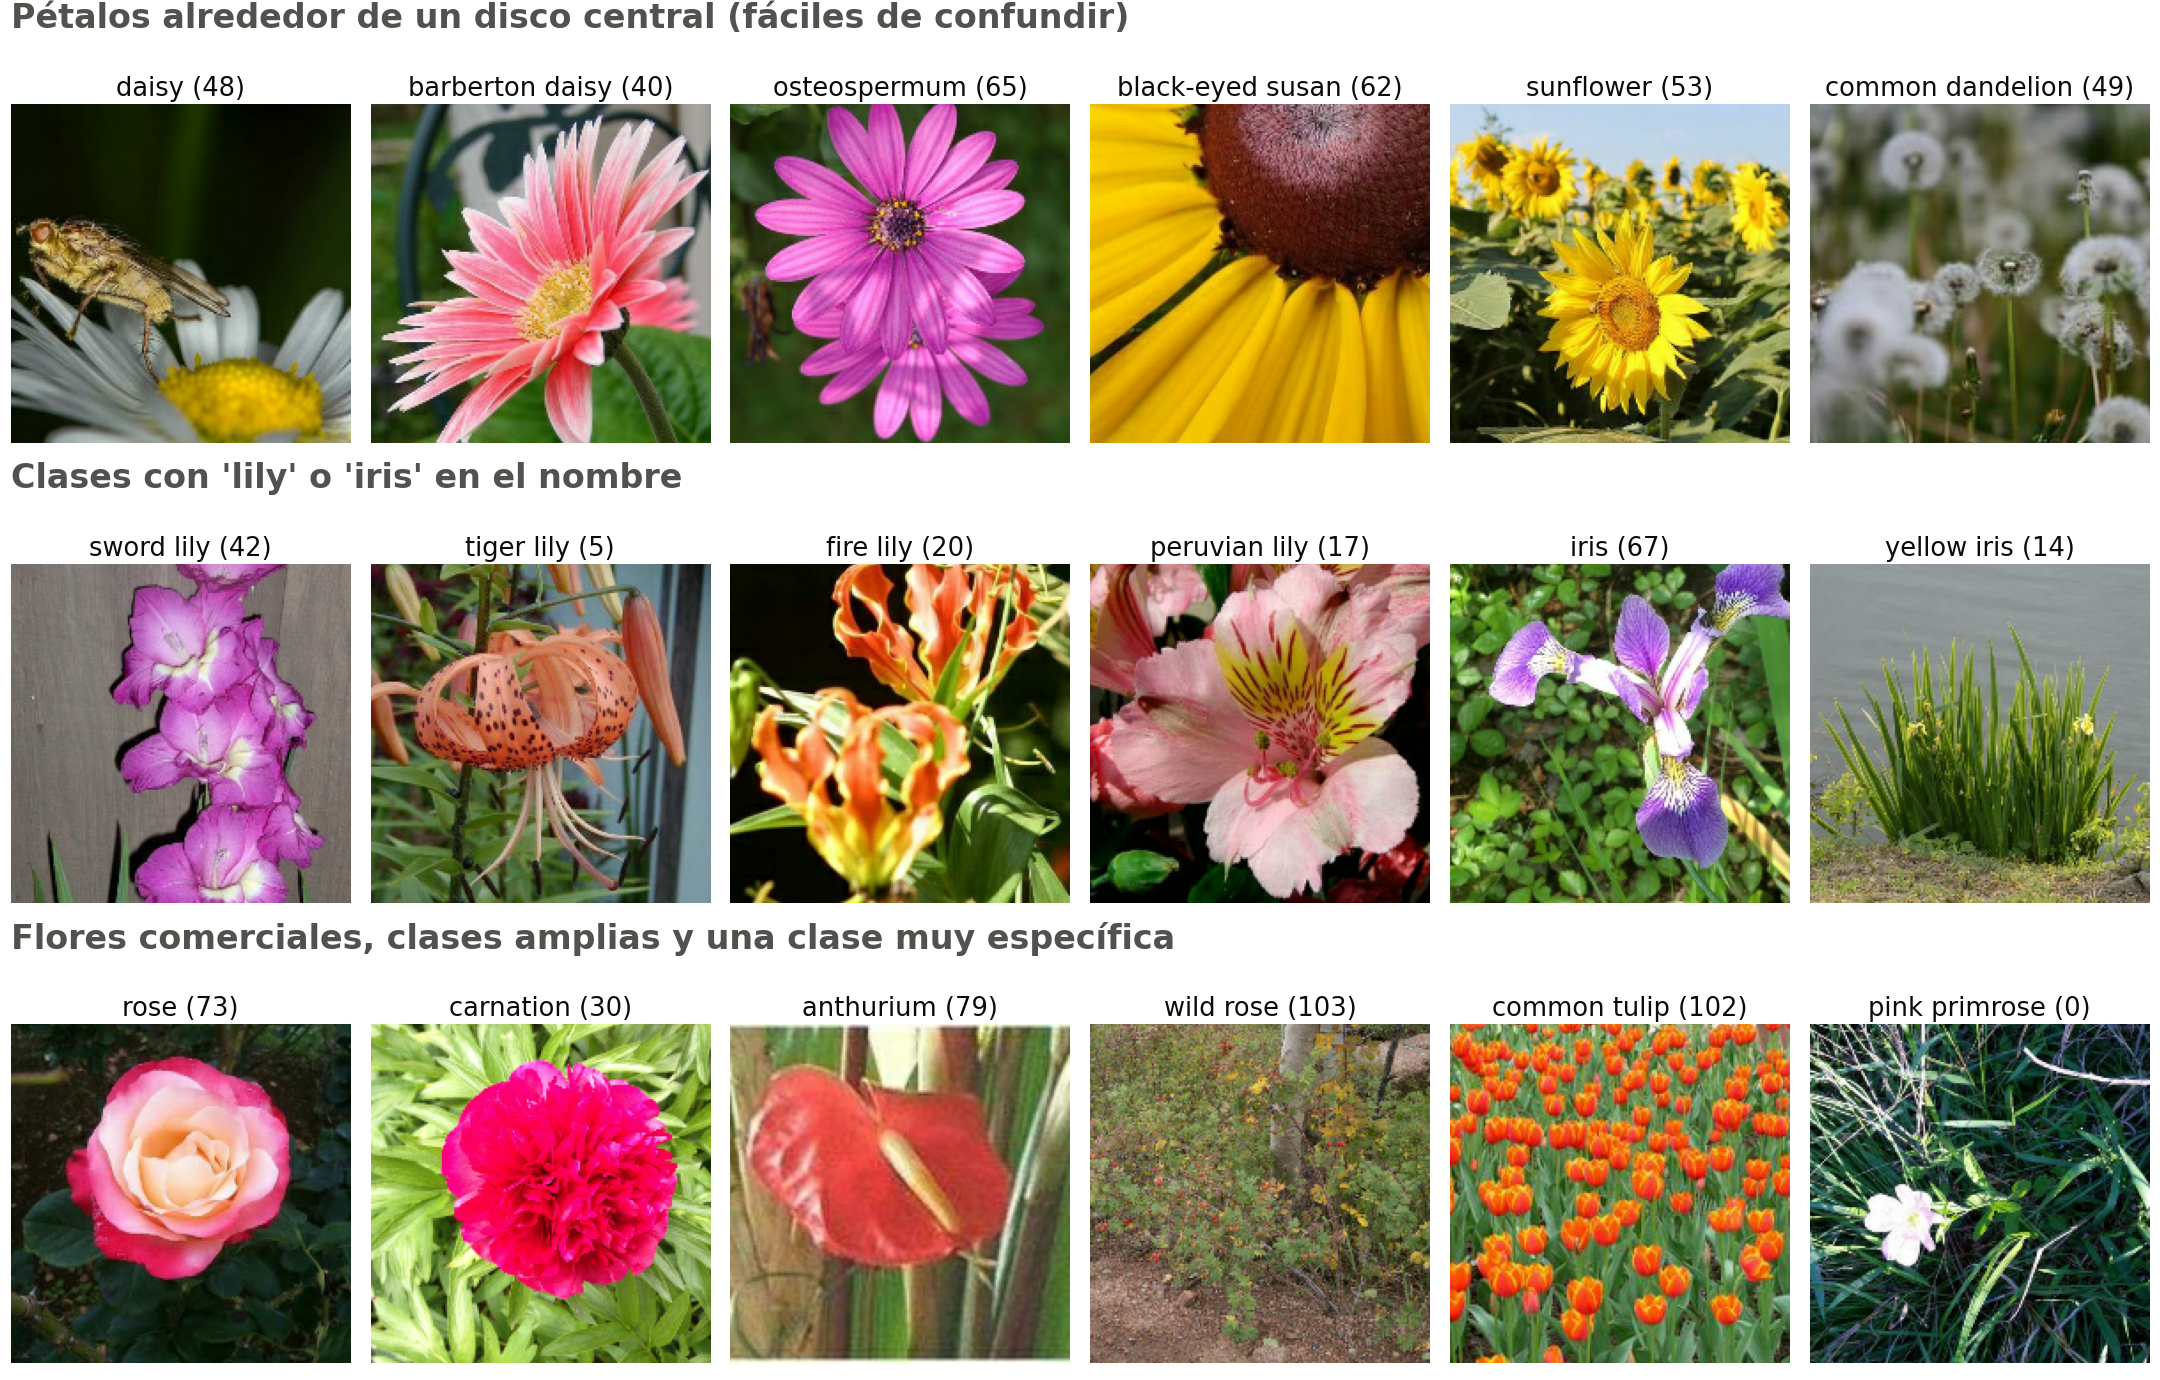
\includegraphics[width=\textwidth]{ejemplos_flores.png}
\caption{Ejemplos reales del conjunto de entrenamiento con su clase y número de etiqueta.}
\label{fig:ejemplos}
\end{figure*}

\begin{table*}[htbp]
\centering
\caption{Clases de ejemplo (nombre y etiqueta) más lo que ilustran.}
\label{tab:ejemplos}
\small
\begin{tabular}{p{0.35\textwidth}p{0.58\textwidth}}
\hline
Clase (etiqueta) & Que ilustra \\
\hline
\textit{sunflower} (53) & Girasol. Flor grande y muy característica. Posiblemente sea de las más fáciles de identificar. \\
\textit{daisy} (48), \textit{barberton daisy} (40), \textit{osteospermum} (65), \textit{black-eyed susan} (62) & Margarita, gerbera, osteospermum y rudbeckia. Todas tienen pétalos alrededor de un disco central. Pueden surgir confusiones entre ellas. \\
\textit{sword lily} (42), \textit{tiger lily} (5), \textit{fire lily} (20), \textit{peruvian lily} (17) & Gladiola, lirio tigre, gloriosa y alstroemeria. Todas dicen \textit{lily}, pero son de cuatro familias botánicas distintas: el modelo tiene que fijarse en la forma, no en el nombre. \\
\textit{iris} (67), \textit{yellow iris} (14) & Misma forma general, la diferencia principal es el color. \\
\textit{rose} (73), \textit{wild rose} (103) & Dos clases de rosas. \textit{Wild rose} es amplia (varias subvariedades) y no viene de Oxford 102. \\
\textit{common tulip} (102) & Tulipán. Clase amplia que tampoco viene de Oxford 102. \\
\textit{pink primrose} (0) & Clase muy específica con un solo subtipo de flor. \\
\textit{carnation} (30) & Clavel, una de las flores comerciales que se producen en el Estado de México. \\
\hline
\end{tabular}
\end{table*}


\subsection{Balance de clases y métrica de evaluación}
Con 12,753 imágenes de entrenamiento y 104 clases, tenemos en promedio 123 imágenes por clase ($12{,}753/104 \approx 122.6$). Sin embargo, las clases no tienen el mismo tamaño: como unas clases agrupan muchas subvariedades y otras solo una, algunas tienen muchas más imágenes que otras.

Por este desbalance, la exactitud no basta: un modelo puede acertar mucho en las clases grandes, fallar en las clases pequeñas y aún verse bien. Por esto mismo, Kaggle califica con el F1 macro \citep{kagglePetalsMetal}. Para cada clase $c$ se calcula la precisión $P_c$, la sensibilidad (\textit{recall}) $R_c$ y su media armónica:

\begin{equation}
P_c=\frac{TP_c}{TP_c+FP_c}, \quad R_c=\frac{TP_c}{TP_c+FN_c},
\end{equation}
\begin{equation}
F1_c=\frac{2\,P_c\,R_c}{P_c+R_c}, \qquad F1_{\text{macro}}=\frac{1}{104}\sum_{c=0}^{103}F1_c,
\end{equation}
donde $TP_c$, $FP_c$ y $FN_c$ son los verdaderos positivos, falsos positivos, y falsos negativos de la clase $c$ . Así todas las clases pesan lo mismo, sin importar cuántas imágenes tengan. 

\subsection{Implicaciones para el proyecto}
Como Kaggle ya separa entrenamiento y validación, no hizo falta crear una partición propia: entrenamos con \texttt{train} y elegimos y evaluamos modelos e hiperparámetros con \texttt{val}. El conjunto \texttt{test} no se usó, porque no trae etiquetas y no se enviaron predicciones a Kaggle. Las imágenes vienen en JPEG con valores de 0 a 255, por lo que se decodifican y se escalan a $[0,1]$ (Sección~\ref{sec:metodologia}). Como las etiquetas son enteros, cada red produce 104 valores de salida, uno por clase, que se convierten en probabilidades con Softmax, y se entrena con entropía cruzada categórica dispersa.

\section{Algoritmos y aplicaciones}
\label{sec:algoritmos}

Dado el problema planteado, su solución implica el uso de algoritmos de visión
por computadora que permitan automatizar la identificación de flores, como en
las aplicaciones descritas en la sección de contexto. A continuación se explica
por qué los algoritmos clásicos no son adecuados y qué arquitecturas proponemos.

\subsection{Algoritmos clásicos de aprendizaje automático}

Algoritmos como $k$ vecinos más cercanos (KNN), \textit{Random Forest} (RF) y
máquinas de soporte vectorial (SVM) funcionan de manera correcta con datos
tabulares, pero se adaptan mal a imágenes. Una imagen de $224\times224$ píxeles
RGB tiene $224\cdot224\cdot3 = 150{,}528$ valores, y una de $112\times112$, la
resolución que usamos, tiene 37,632. Tratar cada valor como una característica
independiente genera varios problemas:

\begin{itemize}
\item \textbf{KNN.} En espacios con tantas dimensiones, las distancias entre
puntos dejan de ser informativas (la llamada maldición de la dimensionalidad).
Además, la distancia entre píxeles no refleja similitud visual: dos fotos de la
misma flor con un ligero desplazamiento o distinta iluminación quedan muy lejos
entre sí. KNN guarda todo el conjunto de entrenamiento y calcula distancias
contra todas las imágenes en cada predicción, lo cual es costoso.
\item \textbf{Random Forest.} Cada árbol divide los datos según el valor de un
solo píxel, sin considerar su posición relativa ni sus vecinos, por lo que no
puede capturar formas ni texturas.
\item \textbf{SVM.} Con kernel, el costo de entrenamiento crece rápidamente con
el número de imágenes y de dimensiones, y sobre píxeles crudos no es invariante
a desplazamientos, rotaciones ni cambios de escala, que en este conjunto son
comunes.
\end{itemize}

Estos métodos requerirían extraer características manualmente (bordes, color,
textura) antes de clasificar. Las redes convolucionales evitan este paso, ya que
aprenden las características directamente de los píxeles.

\begin{figure}[htbp]
    \centering
    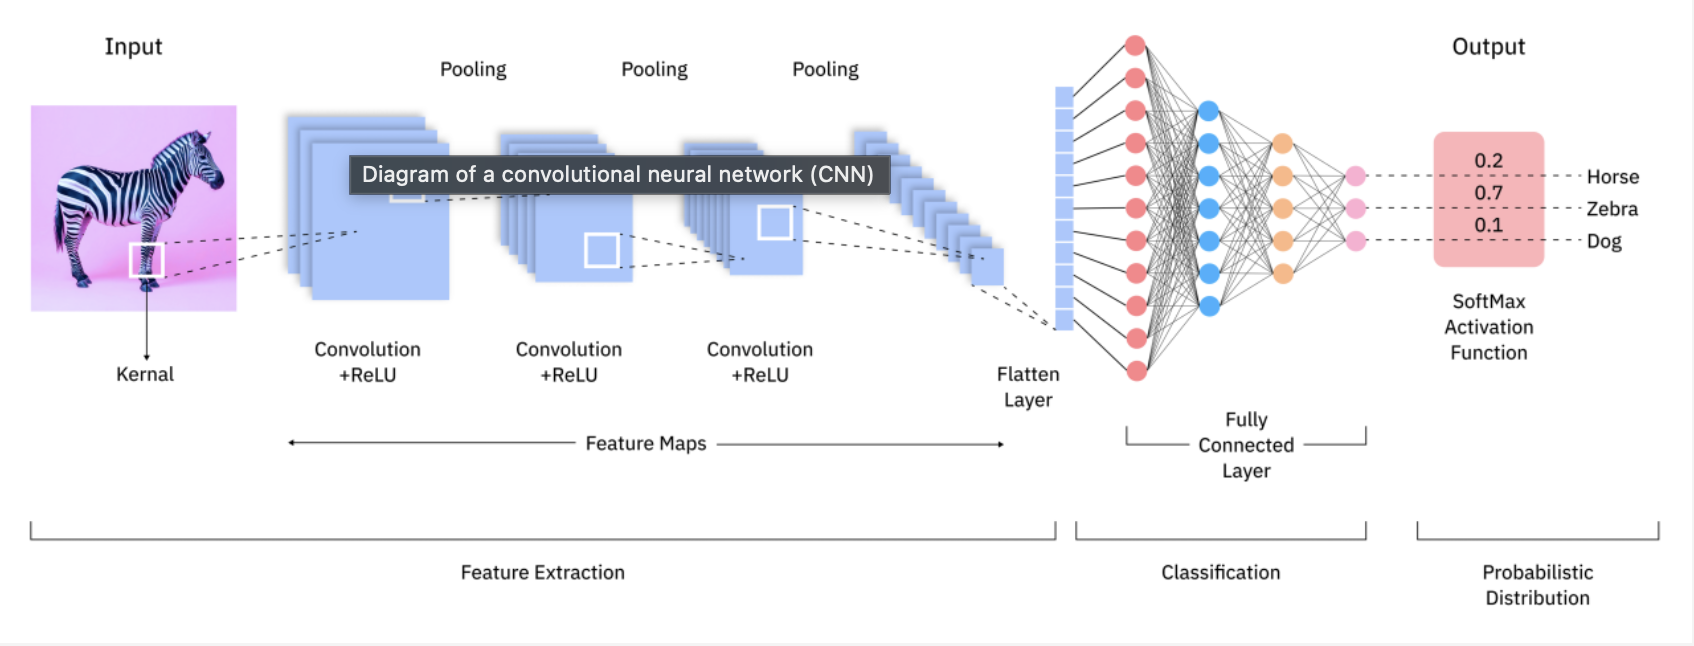
\includegraphics[width=\columnwidth]{cnn_diagram.png}
    \caption{Esquema de una red convolucional: las convoluciones extraen
    características de la imagen y las capas densas las usan para clasificar
    \autocite{ibmWhatImage}.}
    \label{fig:cnn_diagram}
\end{figure}

\subsection{CNN propia entrenada desde cero}
\label{sec:cnn-propia}

Las redes neuronales convolucionales (CNN) son una alternativa especialmente
adecuada para este problema debido a su capacidad para procesar información
espacial (Figura~\ref{fig:cnn_diagram}). Mediante filtros convolucionales pueden
aprender automáticamente características de las imágenes, como bordes, texturas
y formas. En las capas internas pueden emplearse funciones de activación como
ReLU, mientras que Softmax puede utilizarse en la salida para representar las
probabilidades de las distintas clases.

Nuestra primera propuesta es una CNN propia con cuatro bloques convolucionales
(de 32 a 256 filtros), \textit{Global Average Pooling}, una capa densa de 256
neuronas con \textit{dropout} de 0.5 y una capa de salida \textit{softmax} de
104 neuronas. Tiene 480,936 parámetros entrenables
(Tabla~\ref{tab:parametros}) y recibe imágenes de $112\times112$ píxeles.

Elegimos empezar desde cero por tres razones. Es ligera: se entrena en unos 20
minutos en una GPU de una Mac M4, lo que permite repetir experimentos. Permite
estudiar de forma controlada el efecto de la regularización, de la profundidad
y del desbalance, porque todo lo que la red sabe lo aprende de estos datos. Y
sirve como línea base para medir cuánto aportaría un modelo preentrenado. Su
reto es que, con un promedio de solo 123 imágenes por clase, existe riesgo de
sobreajuste, tema que se mide en la Sección~\ref{sec:res-regularizacion}.

\subsection{Transferencia de aprendizaje}
\label{sec:transfer}

La segunda alternativa es partir de una red ya entrenada en ImageNet
\autocite{deng2009imagenet}, con 1.2 millones de imágenes de 1,000 categorías, y
ajustarla a las flores. Dos arquitecturas concretas son adecuadas:

\begin{itemize}
\item \textbf{ResNet50} \autocite{he2016resnet}: 50 capas con conexiones
residuales, que suman la entrada de cada bloque a su salida. Esto permite
entrenar redes muy profundas sin que el gradiente se desvanezca. Tiene unos 25
millones de parámetros y usa entradas de $224\times224$.
\item \textbf{EfficientNetB0} \autocite{tan2019efficientnet}: escala de forma
equilibrada la profundidad, el ancho y la resolución de la red. Con unos 5.3
millones de parámetros y entradas de $224\times224$ logra una exactitud en
ImageNet comparable a la de ResNet50 con cinco veces menos parámetros.
\end{itemize}

Estas redes sirven con unas 123 imágenes por clase porque no aprenden desde
cero: sus primeras capas ya detectan bordes, texturas y formas generales, y
solo hace falta ajustar las últimas capas (o reemplazar la de salida) para
distinguir las 104 clases. Así, la poca información por clase se usa para
aprender lo específico de cada flor y no lo general de una imagen. Además, su
entrada de $224\times224$ coincide con una de las resoluciones del conjunto y
conserva detalles que se pierden a $112\times112$.

Conviene probar la transferencia de aprendizaje cuando la CNN propia deja de
mejorar con más regularización o capacidad, que es lo que muestran los
resultados de este trabajo (Sección~\ref{sec:analisis}). El repositorio ya
incluye la configuración para EfficientNetB0, pero su corrida no se completó
por tiempo de cómputo, por lo que queda como trabajo futuro.

\subsection{Aplicaciones y alcance}

Un modelo como el de este trabajo podría integrarse en una aplicación que, a
partir de una fotografía, sugiera la flor más probable y sus alternativas, al
estilo de iNaturalist \autocite{inaturalist}, o en herramientas educativas para
jardines botánicos y escuelas. En ambos casos funcionaría como apoyo a una
persona y no como identificación definitiva.

Cabe aclarar que el modelo solo puede reconocer las 104 clases presentes en el
conjunto de datos: ante una flor de otra especie, elegirá la más parecida de
esas 104. Una aplicación real más amplia requeriría entrenarlo con una variedad
mucho mayor de especies y detectar cuándo una imagen no pertenece a ninguna
clase conocida.

\section{Metodología}
\label{sec:metodologia}

\subsection{Representación de las arquitecturas implementadas}

La Figura~\ref{fig:arquitecturas-av4} representa los tres diseños entrenados
desde cero. La entrada efectiva es una imagen RGB de $112\times112$ píxeles,
obtenida de los TFRecord de $224\times224$ mediante redimensionamiento bilineal
con antialias.

\begin{figure*}[p]
\centering
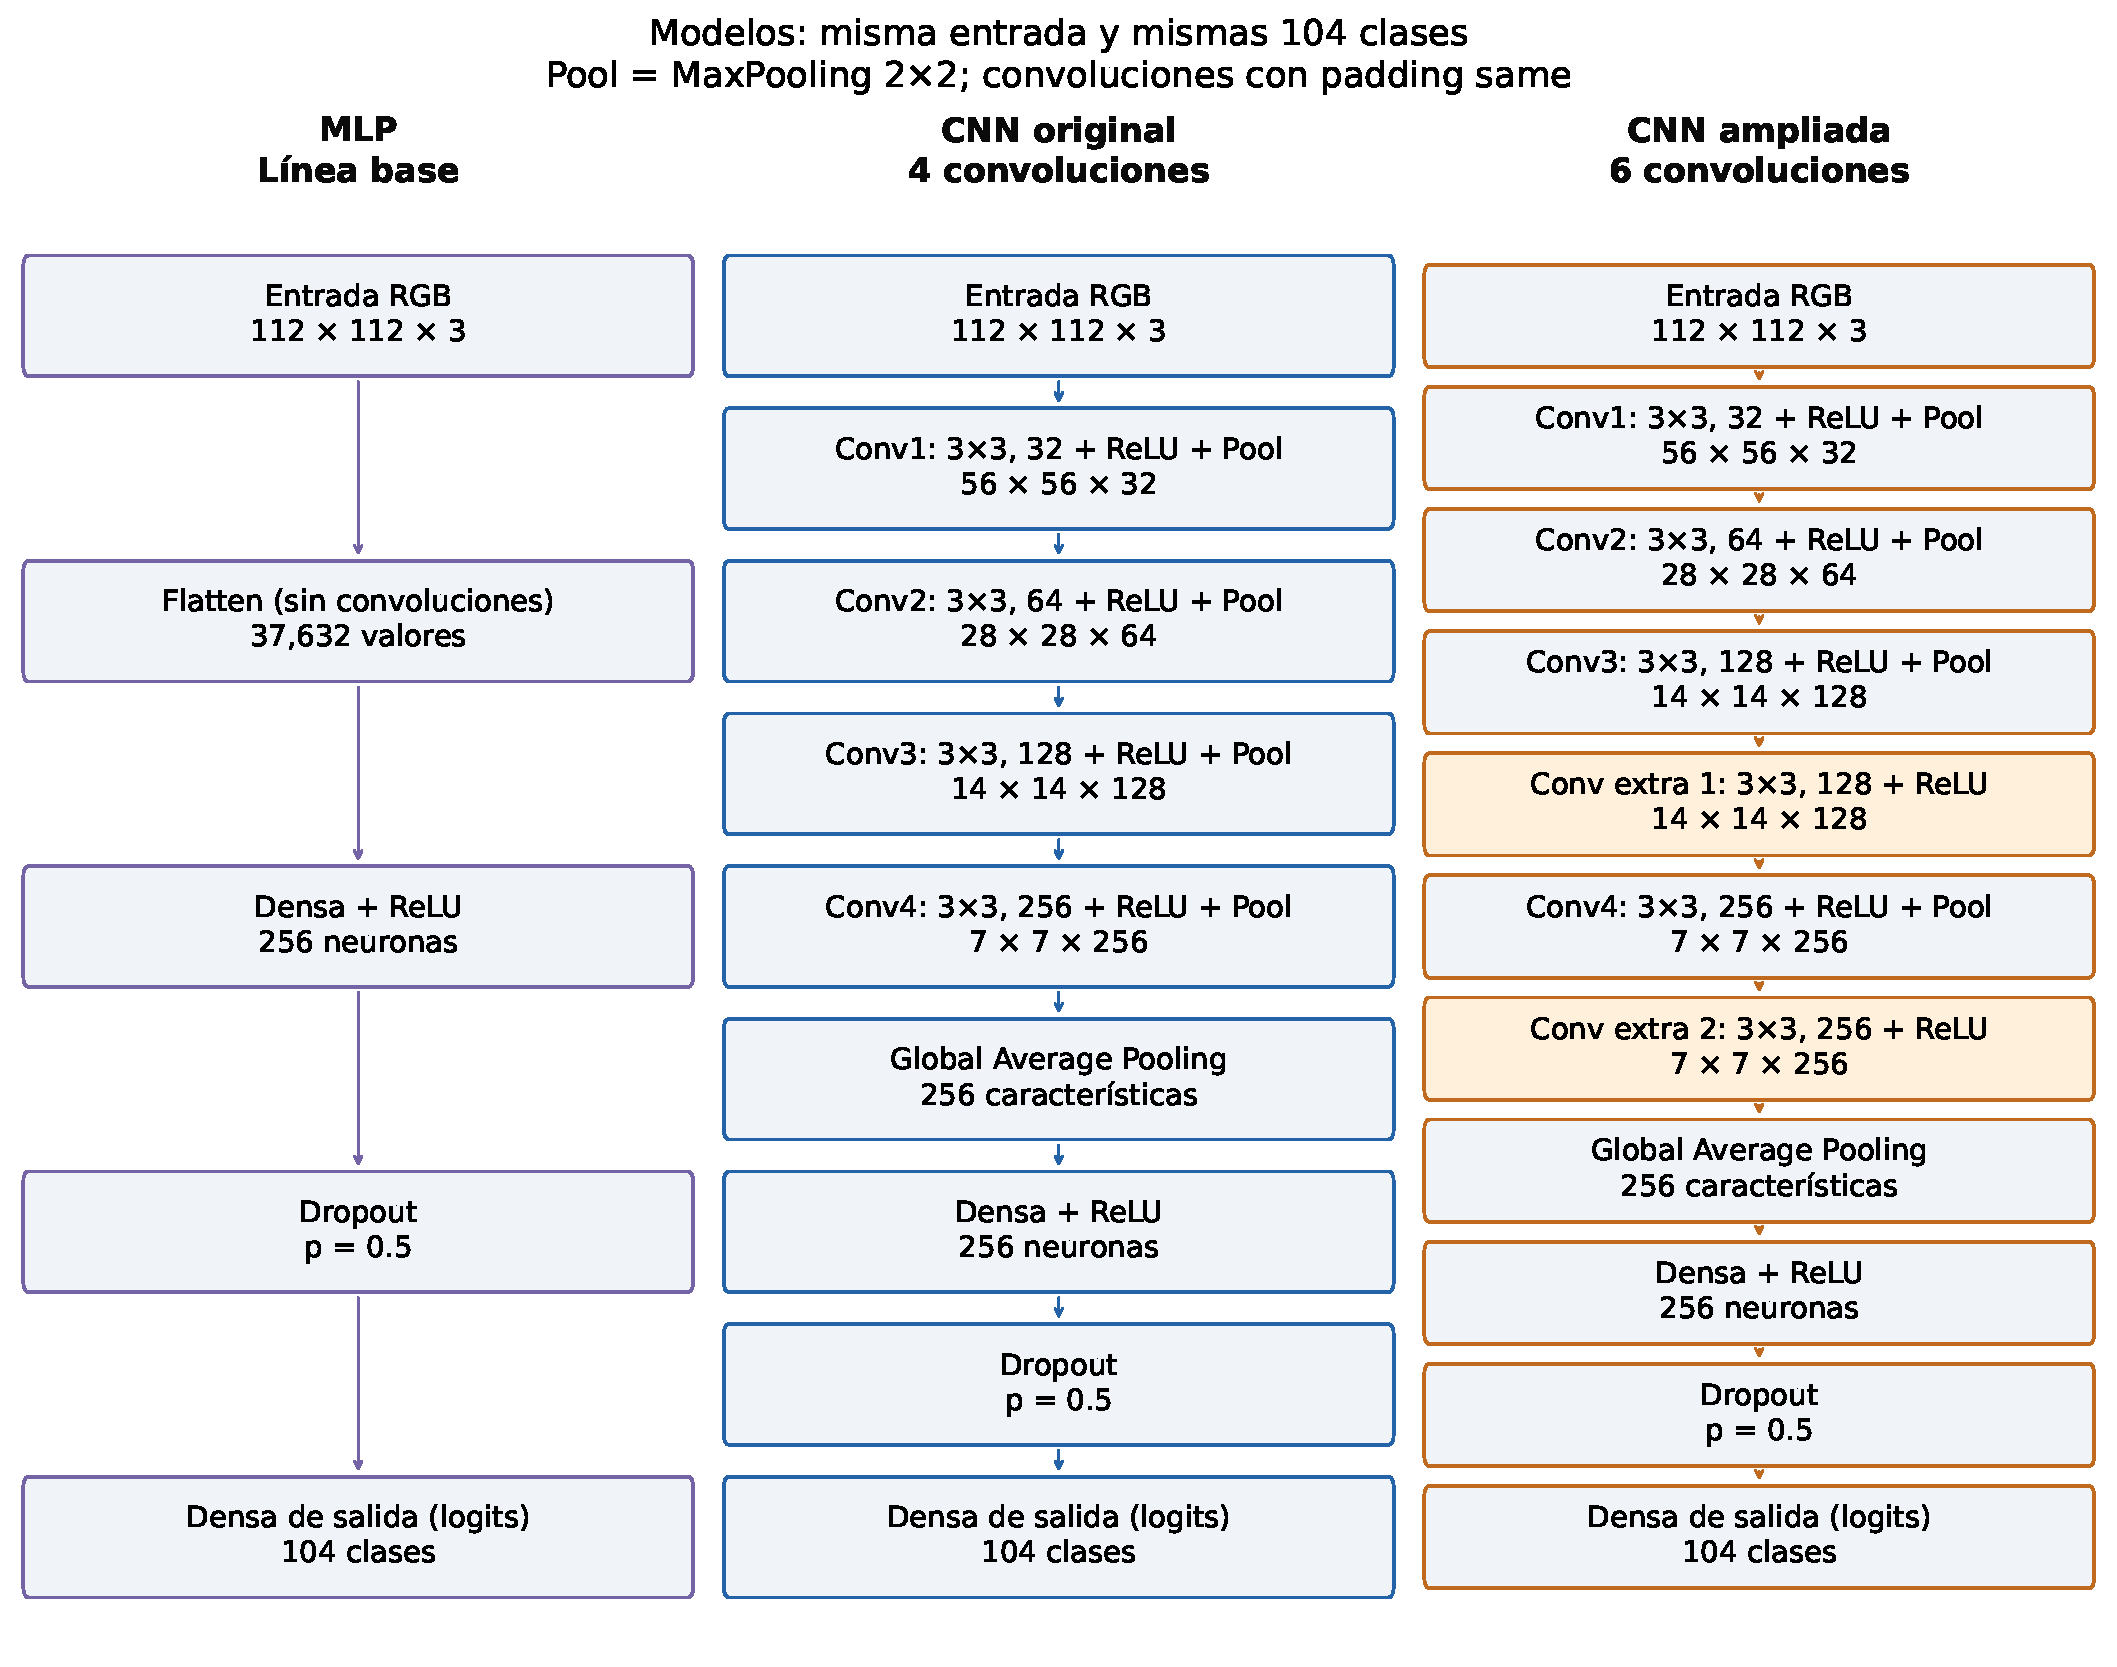
\includegraphics[width=\textwidth,height=0.85\textheight,keepaspectratio]{arquitecturas.pdf}
\caption{Representación de la red totalmente conectada de referencia, la CNN
original y la CNN con dos convoluciones adicionales. Las dimensiones corresponden
a las salidas de cada etapa; las capas adicionales se destacan en naranja.
La variante regularizada conserva la arquitectura de la CNN original.}
\label{fig:arquitecturas-av4}
\end{figure*}

La red \textbf{totalmente conectada de referencia} aplana los $112\times112\times3$
valores de entrada en un vector de 37,632 componentes. Aplica una capa densa de
256 unidades con ReLU, dropout \autocite{srivastava2014dropout} de 0.5 y una salida de 104 logits. No contiene
convoluciones ni pooling. Utiliza el mismo cargador, aumentos y ciclo de entrenamiento que la CNN.

La \textbf{CNN original} emplea cuatro convoluciones de $3\times3$, padding
\textit{same}, ReLU y 32, 64, 128 y 256 filtros. Cada convolución va seguida de
max pooling de $2\times2$. Las salidas de esos bloques son
$56\times56\times32$, $28\times28\times64$, $14\times14\times128$ y
$7\times7\times256$. Después aplica global average pooling (GAP), una capa densa
de 256 unidades con ReLU, dropout de 0.5 y 104 logits de salida.

La \textbf{CNN ampliada} agrega dos capas convolucionales ocultas: una de 128
filtros después del tercer pooling y otra de 256 después del cuarto. Ambas usan
kernel $3\times3$, padding \textit{same} y ReLU, sin pooling adicional. Por tanto,
esta versión tiene seis convoluciones. No se trata de dos capas densas nuevas.

La Tabla~\ref{tab:parametros} desglosa los parámetros por capa. En una
convolución de $3\times3$ con $C_{\text{in}}$ canales de entrada y
$C_{\text{out}}$ filtros hay $(9\,C_{\text{in}}+1)\,C_{\text{out}}$ parámetros, y
en una capa densa $(n_{\text{in}}+1)\,n_{\text{out}}$; el pooling no tiene
parámetros. En la CNN original, el 61\% de los parámetros está en la última
convolución, y las dos capas extra de la ampliada (737,664 parámetros) más que
duplican el total. En la MLP, en cambio, la primera capa densa concentra
$(37{,}632+1)\times256 = 9{,}634{,}048$ parámetros, el 99.7\% del total.

\begin{table}[htbp]
\centering
\caption{Parámetros entrenables por capa de las dos CNN.}
\label{tab:parametros}
\small
\setlength{\tabcolsep}{4pt}
\begin{tabular}{llrr}
\toprule
Capa & Salida & Original & Ampliada \\
\midrule
Conv 32 & $112\times112\times32$ & 896 & 896 \\
Conv 64 & $56\times56\times64$ & 18,496 & 18,496 \\
Conv 128 & $28\times28\times128$ & 73,856 & 73,856 \\
Conv 128 (extra) & $14\times14\times128$ & -- & 147,584 \\
Conv 256 & $14\times14\times256$ & 295,168 & 295,168 \\
Conv 256 (extra) & $7\times7\times256$ & -- & 590,080 \\
Densa 256 & 256 & 65,792 & 65,792 \\
Salida & 104 & 26,728 & 26,728 \\
\midrule
Total & & 480,936 & 1,218,600 \\
\bottomrule
\end{tabular}
\par\smallskip
\parbox{0.95\columnwidth}{\footnotesize Todas las convoluciones son de $3\times3$; la densa va después del GAP. Cada convolución va seguida de max pooling de $2\times2$ (sin parámetros), salvo las dos extra. La salida indicada es la de la convolución, antes del pooling.}
\end{table}

La convolución comparte los pesos del filtro entre posiciones y analiza
vecindarios de píxeles. Así puede aprender bordes, texturas y partes de pétalos
antes de combinarlos. Una capa densa sobre píxeles aplanados asigna pesos
independientes a cada posición y no impone esta estructura local. Esta diferencia
motiva la comparación, pero la mejora debe comprobarse con las métricas.

\subsection{Preprocesamiento y aumento de datos}

Se decodifica cada JPEG como RGB, se convierten sus valores a float32, se
normalizan mediante $x_{\mathrm{norm}}=x/255$ y se redimensionan a $112\times112$.
Las etiquetas son enteros entre 0 y 103. Se mantiene la separación de archivos
original entre entrenamiento y validación, sin incorporar imágenes de validación
al entrenamiento.

Solo en entrenamiento se aplican volteo horizontal, rotación aleatoria de factor
0.05, zoom de 0.1 y contraste de 0.1. Los valores resultantes se recortan a $[0,1]$.
Los aumentos se calculan después de la caché y del mezclado, por lo que cambian
entre épocas. La validación usa imágenes deterministas sin aumentos.

\subsection{Pérdida y actualización de parámetros}

Los modelos producen 104 logits $z_k$. La entropía cruzada se calcula directamente
sobre ellos, sin añadir una segunda softmax a la pérdida:
\begin{equation}
L=-\log\left(\frac{\exp(z_c)}{\sum_{k=1}^{104}\exp(z_k)}\right),
\end{equation}
donde $c$ es la clase verdadera. Para visualizar la confianza se transforma la
salida mediante softmax; esta confianza no constituye una evaluación de calibración.

Todas las redes se optimizan con AdamW \autocite{loshchilov2019adamw}
(decaimiento de pesos desacoplado de 0.01, sin aplicarlo a los sesgos) y una
tasa inicial de $10^{-3}$ que se reduce a la mitad cuando la pérdida de
validación no mejora en dos épocas, hasta $10^{-5}$. La MLP es la excepción en
la tasa: usa $10^{-4}$ (mínimo $10^{-6}$), porque en el Avance~4 un primer
intento con $10^{-3}$ colapsó a predecir una sola clase. Todos los modelos usan
lotes de 64 imágenes y se entrenan con TensorFlow~2.18 sobre la GPU de una Mac
M4 (\texttt{tensorflow-metal}).

\subsection{Pesos por clase}
\label{sec:pesos}

Para contrarrestar el desbalance (Sección~\ref{sec:desbalance}), una variante
pondera la pérdida de cada imagen según su clase \autocite{he2009imbalanced}:
\begin{equation}
w_c = \frac{N}{K\,n_c},
\end{equation}
donde $N=12{,}753$ es el total de imágenes, $K=104$ el número de clases y $n_c$
las imágenes de la clase $c$. Una clase de tamaño promedio recibe peso 1; las
clases de 18 imágenes reciben 6.8 y \emph{iris} (782) recibe 0.16. Como
$\sum_c w_c n_c = N$, la escala total de la pérdida no cambia.

\section{Protocolo experimental}

\subsection{Condiciones comunes}

Todos los experimentos usan los mismos 12,753 ejemplos de entrenamiento y 3,712
de validación de las 104 clases, la semilla 0 y lotes de 64 imágenes. La
\emph{referencia} es la CNN de cuatro convoluciones elegida en el Avance~4:
dropout de 0.5 antes de la salida, aumento de datos solo en entrenamiento
(volteo horizontal, rotación, zoom y contraste), AdamW con decaimiento de pesos
de 0.01 \autocite{loshchilov2019adamw}, tasa inicial de $10^{-3}$ reducida a la
mitad cuando la pérdida de validación no mejora en dos épocas (mínimo
$10^{-5}$), entrada de $112\times112$ y hasta 150 épocas. El entrenamiento se
detiene tras 12 evaluaciones sin mejorar el F1 macro de validación y se conserva
el checkpoint con mayor F1 macro; todas las métricas reportadas corresponden a
ese checkpoint, no a la última época.

\subsection{Un cambio a la vez}

Para atribuir cada diferencia a una causa, cada experimento modifica un solo
factor respecto a la referencia: la arquitectura (MLP o CNN ampliada), la pérdida (pesos por clase), la regularización o un
hiperparámetro (tasa de aprendizaje o dropout). Hay dos excepciones declaradas.
La MLP usa una tasa inicial de $10^{-4}$, porque con $10^{-3}$ colapsó a predecir
una sola clase en el Avance~4. La variante \emph{sin regularización} retira a la
vez dropout, aumento y decaimiento de pesos (Adam en lugar de AdamW), para medir
su efecto conjunto.

\subsection{Métricas de entrenamiento comparables con validación}

Las métricas que reporta el ciclo de entrenamiento se calculan con aumento y
dropout activos, por lo que no son comparables con validación. Para medir la
brecha de generalización, en cada época se evalúan además 3,712 imágenes fijas de
entrenamiento (el mismo tamaño que validación) sin aumento y con la red en modo
inferencia. Con ellas se calculan la pérdida, la exactitud y el F1 macro de
entrenamiento. La \emph{brecha F1} es el F1 macro de ese subconjunto menos el de
validación, ambos en la época del checkpoint.

\subsection{Alcance de la evaluación}

La validación se usa para elegir el checkpoint y comparar configuraciones; sus
métricas no son una estimación independiente de generalización. Como el
conjunto de prueba de Kaggle no tiene etiquetas locales, la medida de prueba se
obtiene enviando las predicciones a la competencia
(Sección~\ref{sec:kaggle}). Cada configuración se entrenó con una sola semilla,
por lo que diferencias de pocas milésimas de F1 macro no se interpretan como
mejoras. Los resultados de este documento se generaron con TensorFlow~2.18 en una
GPU Apple M4 (\texttt{tensorflow-metal}); las corridas del Avance~4 se hicieron
con PyTorch/DirectML, por lo que sus cifras no se mezclan con las de este reporte.

\subsection{Reproducibilidad}
\label{sec:repo}

El código, las configuraciones y los resultados están en el repositorio público
\url{https://github.com/Lunaaaalj/NeuralNetworksTeamEnvironment}. El
\texttt{README} explica la instalación y los comandos. El notebook
\path{notebooks/reporte_final.ipynb} reconstruye de principio a fin la tabla de
resultados (\path{reports/final/resultados.csv}), las tablas y las figuras de
este documento, a partir de los \texttt{history.csv}, \texttt{summary.json} y
\texttt{eval\_report.json} versionados de cada experimento; con
\texttt{RUN\_TRAINING = True} también vuelve a entrenarlos. La matriz de
experimentos está en \path{scripts/run_final.py} y la configuración de referencia
en \path{configs/final.yaml}.

\section{Resultados}
\label{sec:resultados}

Todas las cifras de esta sección provienen de
\path{reports/final/resultados.csv}, que el notebook de la
Sección~\ref{sec:repo} reconstruye a partir de los \texttt{history.csv} y
\texttt{eval\_report.json} de cada corrida. Salvo que se indique otra cosa,
las métricas son de validación (3,712 imágenes) en el checkpoint con mayor F1
macro.

\subsection{Desbalance de clases}
\label{sec:desbalance}

El conjunto de entrenamiento tiene 12,753 imágenes repartidas de forma muy
desigual entre las 104 clases (Figura~\ref{fig:distribucion}). La clase más
pequeña tiene 18 imágenes (\emph{moon orchid}, \emph{bolero deep blue} y
\emph{alpine sea holly}) y la más grande 782 (\emph{iris}): una razón de
43:1. La mediana es de 88 imágenes y la media de 122.6; la media queda por
encima de la mediana porque unas pocas clases concentran los datos: las 10 más
grandes reúnen el 40\% de las imágenes, mientras que 24 clases tienen menos de
30. El rango intercuartílico va de 32.5 a 125.5 imágenes. Validación conserva
exactamente las mismas proporciones (de 5 a 228 imágenes por clase), de modo
que las clases raras tienen también muy pocos ejemplos para evaluarlas: el F1
de una clase con 5 imágenes de validación cambia en más de 0.15 con un solo
acierto.

\begin{figure*}[htbp]
\centering
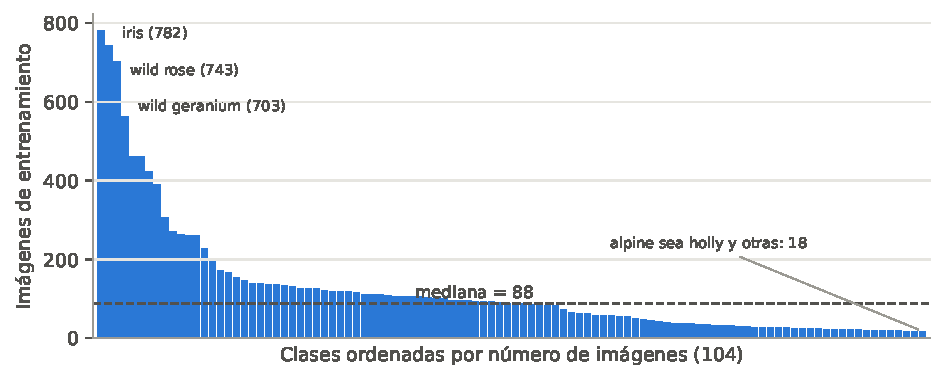
\includegraphics[width=0.85\textwidth]{distribucion_clases.pdf}
\caption{Imágenes de entrenamiento por clase, ordenadas de mayor a menor. La
línea punteada marca la mediana (88).}
\label{fig:distribucion}
\end{figure*}

\subsection{Arquitecturas: MLP, CNN de referencia y CNN ampliada}
\label{sec:res-arquitecturas}

La Tabla~\ref{tab:modelos} resume las arquitecturas y la
Figura~\ref{fig:curvas-modelos} muestra sus curvas de pérdida, exactitud y F1
macro en entrenamiento y validación. La CNN de referencia alcanza un F1 macro de
0.5784 y una exactitud de 64.06\%; la MLP, con 20 veces más parámetros, se
queda en 0.0178 y 14.36\%. La CNN ampliada llega a 0.5663, por debajo de la
referencia. Su corrida se interrumpió en la época 50 por un bloqueo de la GPU;
como su F1 de validación llevaba ocho épocas estable alrededor de 0.564 y la
tasa de aprendizaje ya había bajado a $3\times10^{-5}$, es poco probable que
hubiera alcanzado a la referencia.

\begin{table*}[htbp]
\centering
\caption{Arquitecturas comparadas con los mismos datos de validación (3,712 imágenes).}
\label{tab:modelos}
\small
\begin{tabular}{lrrrrrrr}
\toprule
Modelo & Parámetros & Época & Exact. (\%) & F1 entr. & Brecha F1 & Tiempo (min) & F1 macro \\
\midrule
MLP & 9,660,776 & 62/74 & 14.36 & 0.0192 & +0.0014 & 6.9 & 0.0178 \\
CNN de referencia & 480,936 & 91/103 & 64.06 & 0.8138 & +0.2354 & 19.7 & \textbf{0.5784} \\
CNN ampliada (6 conv.)$^\dagger$ & 1,218,600 & 41/49 & 63.77 & 0.7936 & +0.2273 & 17.1 & 0.5663 \\
\bottomrule
\end{tabular}
\par\smallskip
\parbox{0.95\textwidth}{\footnotesize Época: checkpoint elegido por F1 macro / épocas ejecutadas. F1 entr.: F1 macro sobre 3,712 imágenes fijas de entrenamiento sin aumento ni dropout, en la misma época. Brecha F1 = F1 entr. $-$ F1 macro de validación. Todas a 112$\times$112, entrenadas desde cero con semilla 0. $^\dagger$La corrida se interrumpió en la época 50 por un bloqueo de la GPU; se reporta su mejor checkpoint.}
\end{table*}


\begin{figure*}[htbp]
\centering
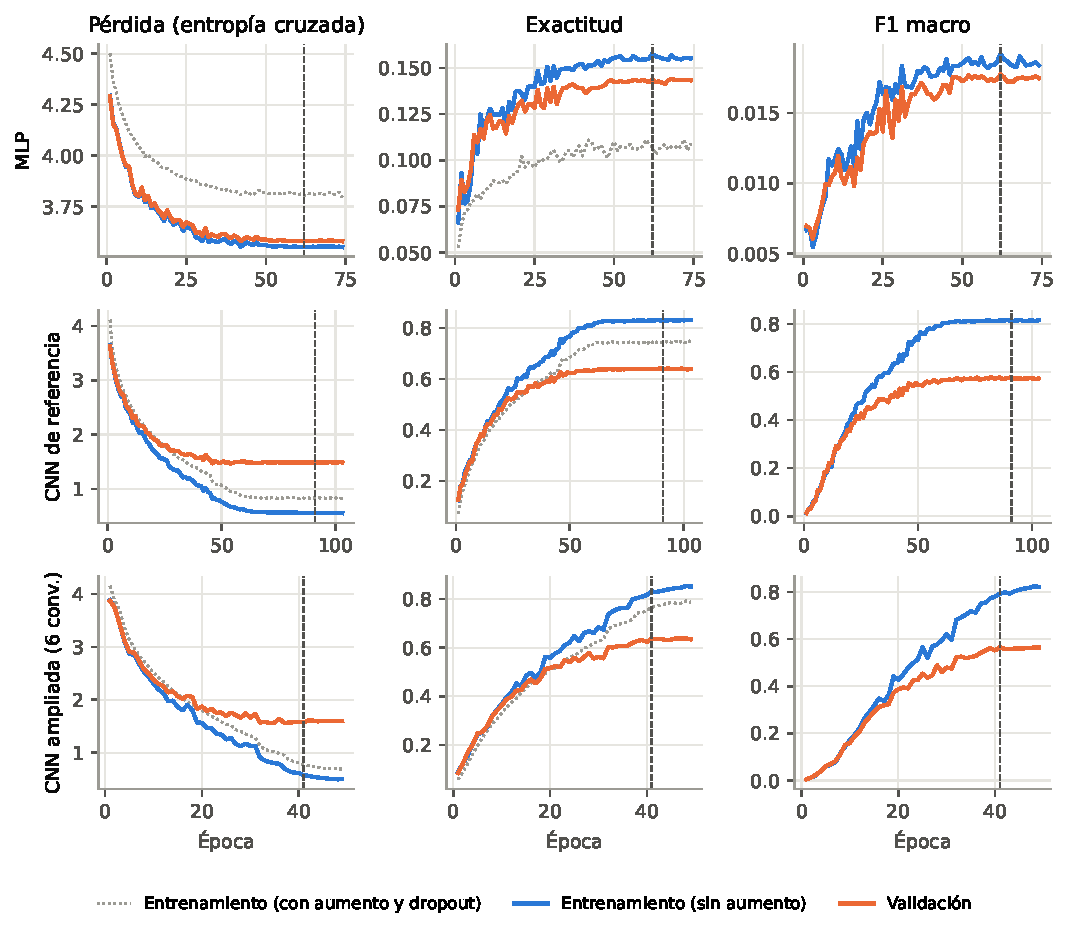
\includegraphics[width=\textwidth]{curvas_modelos.pdf}
\caption{Curvas de entrenamiento y validación por época. Azul: 3,712 imágenes
fijas de entrenamiento sin aumento, en modo inferencia. Naranja: validación.
Gris punteado: la métrica que reporta el ciclo de entrenamiento, con aumento y
dropout activos (no existe para el F1). La línea vertical marca el checkpoint
elegido. Las escalas verticales de la MLP son distintas.}
\label{fig:curvas-modelos}
\end{figure*}

Las curvas muestran tres comportamientos distintos:

\begin{itemize}
\item \textbf{CNN de referencia: sobreajuste moderado y controlado.} Las dos
curvas avanzan juntas durante unas 15 épocas y después se separan. La pérdida de
validación toca su mínimo en la época 54 (1.464) y después apenas sube (1.486 al
final), mientras el F1 de validación sigue mejorando poco a poco hasta
la época 91. En el checkpoint, el F1 de entrenamiento es 0.8138 y el de
validación 0.5784: una brecha de 0.235.
\item \textbf{CNN ampliada: el mismo techo, alcanzado antes.} Con 2.5 veces más
parámetros aprende el entrenamiento más rápido (en la época 41 su F1 de
entrenamiento es 0.794 frente a 0.638 de la referencia), pero su validación se
estanca en el mismo nivel. Su pérdida de validación toca su mínimo antes (época
34) y después sube de 1.555 a 1.602, una señal de sobreajuste más clara que en
la referencia.
\item \textbf{MLP: infraajuste.} Entrenamiento y validación casi coinciden
(brecha de F1 de 0.001) y ambas son muy bajas. La red no memoriza: no logra
aprender. Solo predice 11 de las 104 clases y tiene F1 = 0 en 93.
\end{itemize}

En las tres redes, la curva gris queda por debajo de la azul: el aumento de datos
y el dropout hacen que las métricas del ciclo de entrenamiento parezcan peores
de lo que el modelo realmente rinde sobre imágenes de entrenamiento.

La Tabla~\ref{tab:ultima-epoca} justifica conservar el checkpoint con mayor F1
macro y no la última época. Entre la época 91 y la 103, el modelo sigue
ajustando un poco el entrenamiento (la pérdida baja de 0.557 a 0.551), pero el
F1 de validación cae de 0.5784 a 0.5731 y su pérdida sube. La diferencia entre
exactitud (64.06\%) y F1 macro (0.578) también es informativa: la exactitud
cuenta aciertos sobre todas las imágenes y la dominan las clases grandes; el F1
macro promedia por clase, así que pesa igual una clase de 18 imágenes que
\emph{iris} con 782.

\begin{table}[htbp]
\centering
\caption{CNN de referencia en la época elegida y al terminar el entrenamiento.}
\label{tab:ultima-epoca}
\small
\begin{tabular}{lrr}
\toprule
Métrica & Elegida (91) & Última (103) \\
\midrule
\multicolumn{3}{l}{\textit{Entrenamiento}} \\
\quad Exactitud (\%) & 83.00 & 83.05 \\
\quad F1 macro & 0.8138 & 0.8145 \\
\quad Pérdida & 0.557 & 0.551 \\
\multicolumn{3}{l}{\textit{Validación}} \\
\quad Exactitud (\%) & 64.06 & 63.95 \\
\quad F1 macro & 0.5784 & 0.5731 \\
\quad Pérdida & 1.483 & 1.486 \\
\bottomrule
\end{tabular}
\par\smallskip
\parbox{0.95\columnwidth}{\footnotesize Entre paréntesis, la época. Entrenamiento: 3,712 imágenes fijas sin aumento, en modo inferencia.}
\end{table}


\subsection{Comparación con el Avance~4}

La Tabla~\ref{tab:avance4} contrasta estas corridas con las del Avance~4. El F1
de la referencia se reproduce (0.5745 frente a 0.5784) aunque cambió el
\emph{framework}, lo que da confianza en la comparación. Lo que cambia es la
brecha: medida con aumento y dropout activos, como en el Avance~4, la brecha de
exactitud de la referencia era de 0.105; medida sobre imágenes limpias es de
0.189 en exactitud y de 0.235 en F1 macro. El Avance~4 subestimaba el
sobreajuste a casi la mitad. En la CNN ampliada, que en el Avance~4 se entrenó
con Adam y tasa fija, la misma política de la referencia reduce su desventaja de
0.024 a 0.012 puntos de F1, pero no la elimina.

\begin{table*}[htbp]
\centering
\caption{Avance 4 frente al reporte final: la brecha medida con aumento subestima el sobreajuste.}
\label{tab:avance4}
\small
\begin{tabular}{llrrrrr}
\toprule
Modelo & Política en Avance 4 & F1 A4 & Brecha exact. A4 & F1 final & Brecha exact. & Brecha F1 \\
\midrule
CNN de referencia & AdamW + LR adaptable & 0.5745 & +0.1051 & 0.5784 & +0.1894 & +0.2354 \\
CNN ampliada (6 conv.) & Adam, LR fijo & 0.5502 & +0.1687 & 0.5663 & +0.1926 & +0.2273 \\
MLP & Adam, LR fijo & 0.0280 & -0.0346 & 0.0178 & +0.0140 & +0.0014 \\
\bottomrule
\end{tabular}
\par\smallskip
\parbox{0.95\textwidth}{\footnotesize A4: PyTorch/DirectML; su exactitud de entrenamiento se midió durante el ciclo, con aumento y dropout activos. Final: TensorFlow/Metal, todas con AdamW + LR adaptable; brechas medidas sobre 3,712 imágenes de entrenamiento sin aumento y en modo inferencia, en la época del checkpoint.}
\end{table*}


\subsection{F1 por clase de la CNN de referencia}
\label{sec:por-clase}

El F1 macro de 0.578 esconde mucha variación entre clases
(Tabla~\ref{tab:clases}). La mediana por clase es 0.600; 16 clases superan 0.8 y
13 quedan por debajo de 0.3. Las mejores son flores con forma o color muy
característicos (\emph{pink-yellow dahlia} y \emph{cautleya spicata} con F1 de
1.0, \emph{cape flower} y \emph{purple coneflower} con 0.97). Cinco clases tienen
F1 = 0: \emph{bolero deep blue}, \emph{siam tulip}, \emph{canterbury bells},
\emph{pink quill} y \emph{garden phlox}. Todas tienen entre 18 y 24 imágenes de
entrenamiento y entre 5 y 7 de validación, y el modelo nunca las predice.

\begin{table*}[htbp]
\centering
\caption{F1 por clase de la CNN de referencia: las 10 mejores y las 10 peores.}
\label{tab:clases}
\small
\begin{tabular}{lrrlrr}
\toprule
Mejores & $n_{\text{entr}}$ & F1 & Peores & $n_{\text{entr}}$ & F1 \\
\midrule
pink-yellow dahlia & 58 & 1.000 & bolero deep blue & 18 & 0.000 \\
cautleya spicata & 27 & 1.000 & siam tulip & 19 & 0.000 \\
cape flower & 57 & 0.971 & canterbury bells & 20 & 0.000 \\
purple coneflower & 55 & 0.968 & pink quill & 24 & 0.000 \\
bishop of llandaff & 58 & 0.941 & garden phlox & 24 & 0.000 \\
silverbush & 28 & 0.941 & tree mallow & 29 & 0.154 \\
californian poppy & 55 & 0.938 & sword lily & 63 & 0.200 \\
geranium & 63 & 0.919 & hibiscus & 134 & 0.243 \\
orange dahlia & 36 & 0.900 & spring crocus & 21 & 0.250 \\
osteospermum & 33 & 0.900 & globe-flower & 21 & 0.250 \\
\bottomrule
\end{tabular}
\par\smallskip
\parbox{0.95\textwidth}{\footnotesize $n_{\text{entr}}$: imágenes de esa clase en entrenamiento. Desempates por tamaño de clase.}
\end{table*}


El tamaño de la clase explica solo una parte de estos resultados
(Figura~\ref{fig:f1-tamano}). Las 10 clases más pequeñas tienen un F1 promedio de
0.361 y las 10 más grandes de 0.703, pero la relación no es monótona: las clases
de 30 a 60 imágenes promedian 0.732, más que las de 300 o más (0.690), y la
correlación de Spearman entre tamaño y F1 es apenas 0.12. Los fallos se
concentran en la cola de clases con menos de 30 imágenes (F1 medio 0.461) y en
flores parecidas entre sí. Los pares más confundidos son \emph{carnation}
$\to$ \emph{rose} (13 imágenes), \emph{wild rose} $\to$ \emph{windflower} (12),
\emph{common dandelion} $\to$ \emph{sunflower} (12) y \emph{common tulip}
$\to$ \emph{rose} (11): flores de forma y color similares, donde la clase
predicha suele ser además la más frecuente. La Figura~\ref{fig:confusion} muestra
la matriz de confusión completa.

La Figura~\ref{fig:predicciones} muestra ejemplos reales. Los errores ilustran
en qué se apoya la red: un girasol de pétalos rojos se predice como
\emph{tiger lily} y un iris barbado morado como \emph{wild geranium}, es decir,
cuando el color se aparta del típico de la clase, la red se guía por el color
antes que por la forma. Varios errores tienen además confianza baja (17--42\%),
mientras que los aciertos en clases características (\emph{sunflower},
\emph{iris}) llegan a casi 100\%.

\begin{figure*}[htbp]
\centering
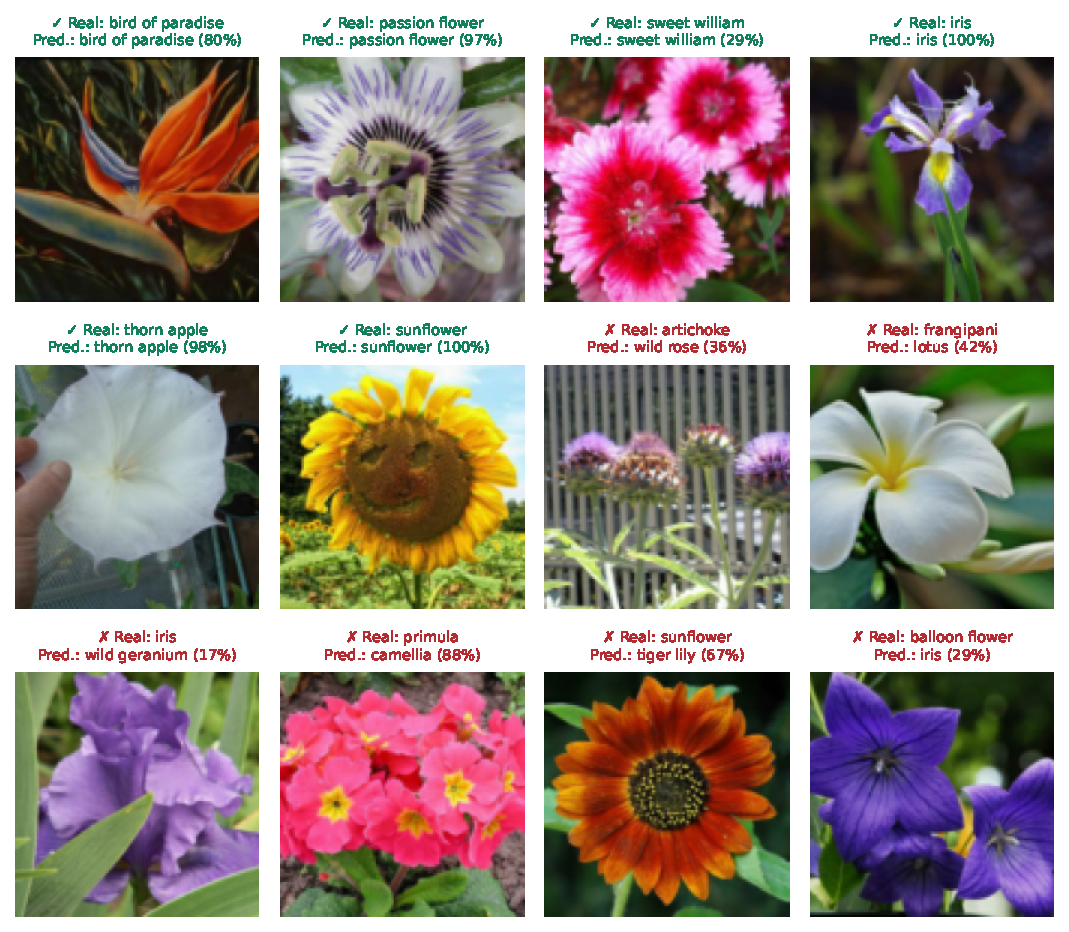
\includegraphics[width=0.8\textwidth]{predicciones_referencia.pdf}
\caption{Seis aciertos (verde, \checkmark) y seis errores (rojo, $\times$) de la
CNN de referencia en validación, elegidos con semilla fija; entre paréntesis, la
probabilidad softmax de la clase predicha. La proporción es ilustrativa: la red
acierta en 2,378 de 3,712 imágenes.}
\label{fig:predicciones}
\end{figure*}

\begin{figure}[htbp]
\centering
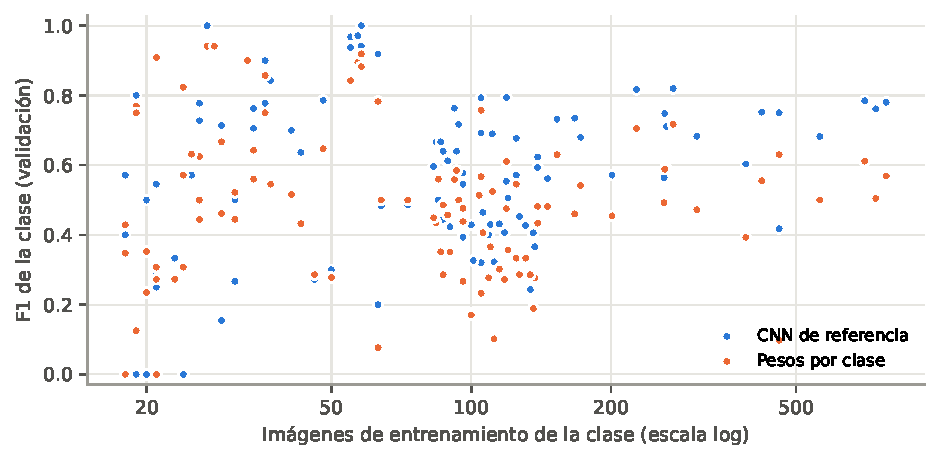
\includegraphics[width=\columnwidth]{f1_vs_tamano_clase.pdf}
\caption{F1 de validación de cada clase frente a su número de imágenes de
entrenamiento (escala logarítmica).}
\label{fig:f1-tamano}
\end{figure}

\begin{figure*}[p]
\centering
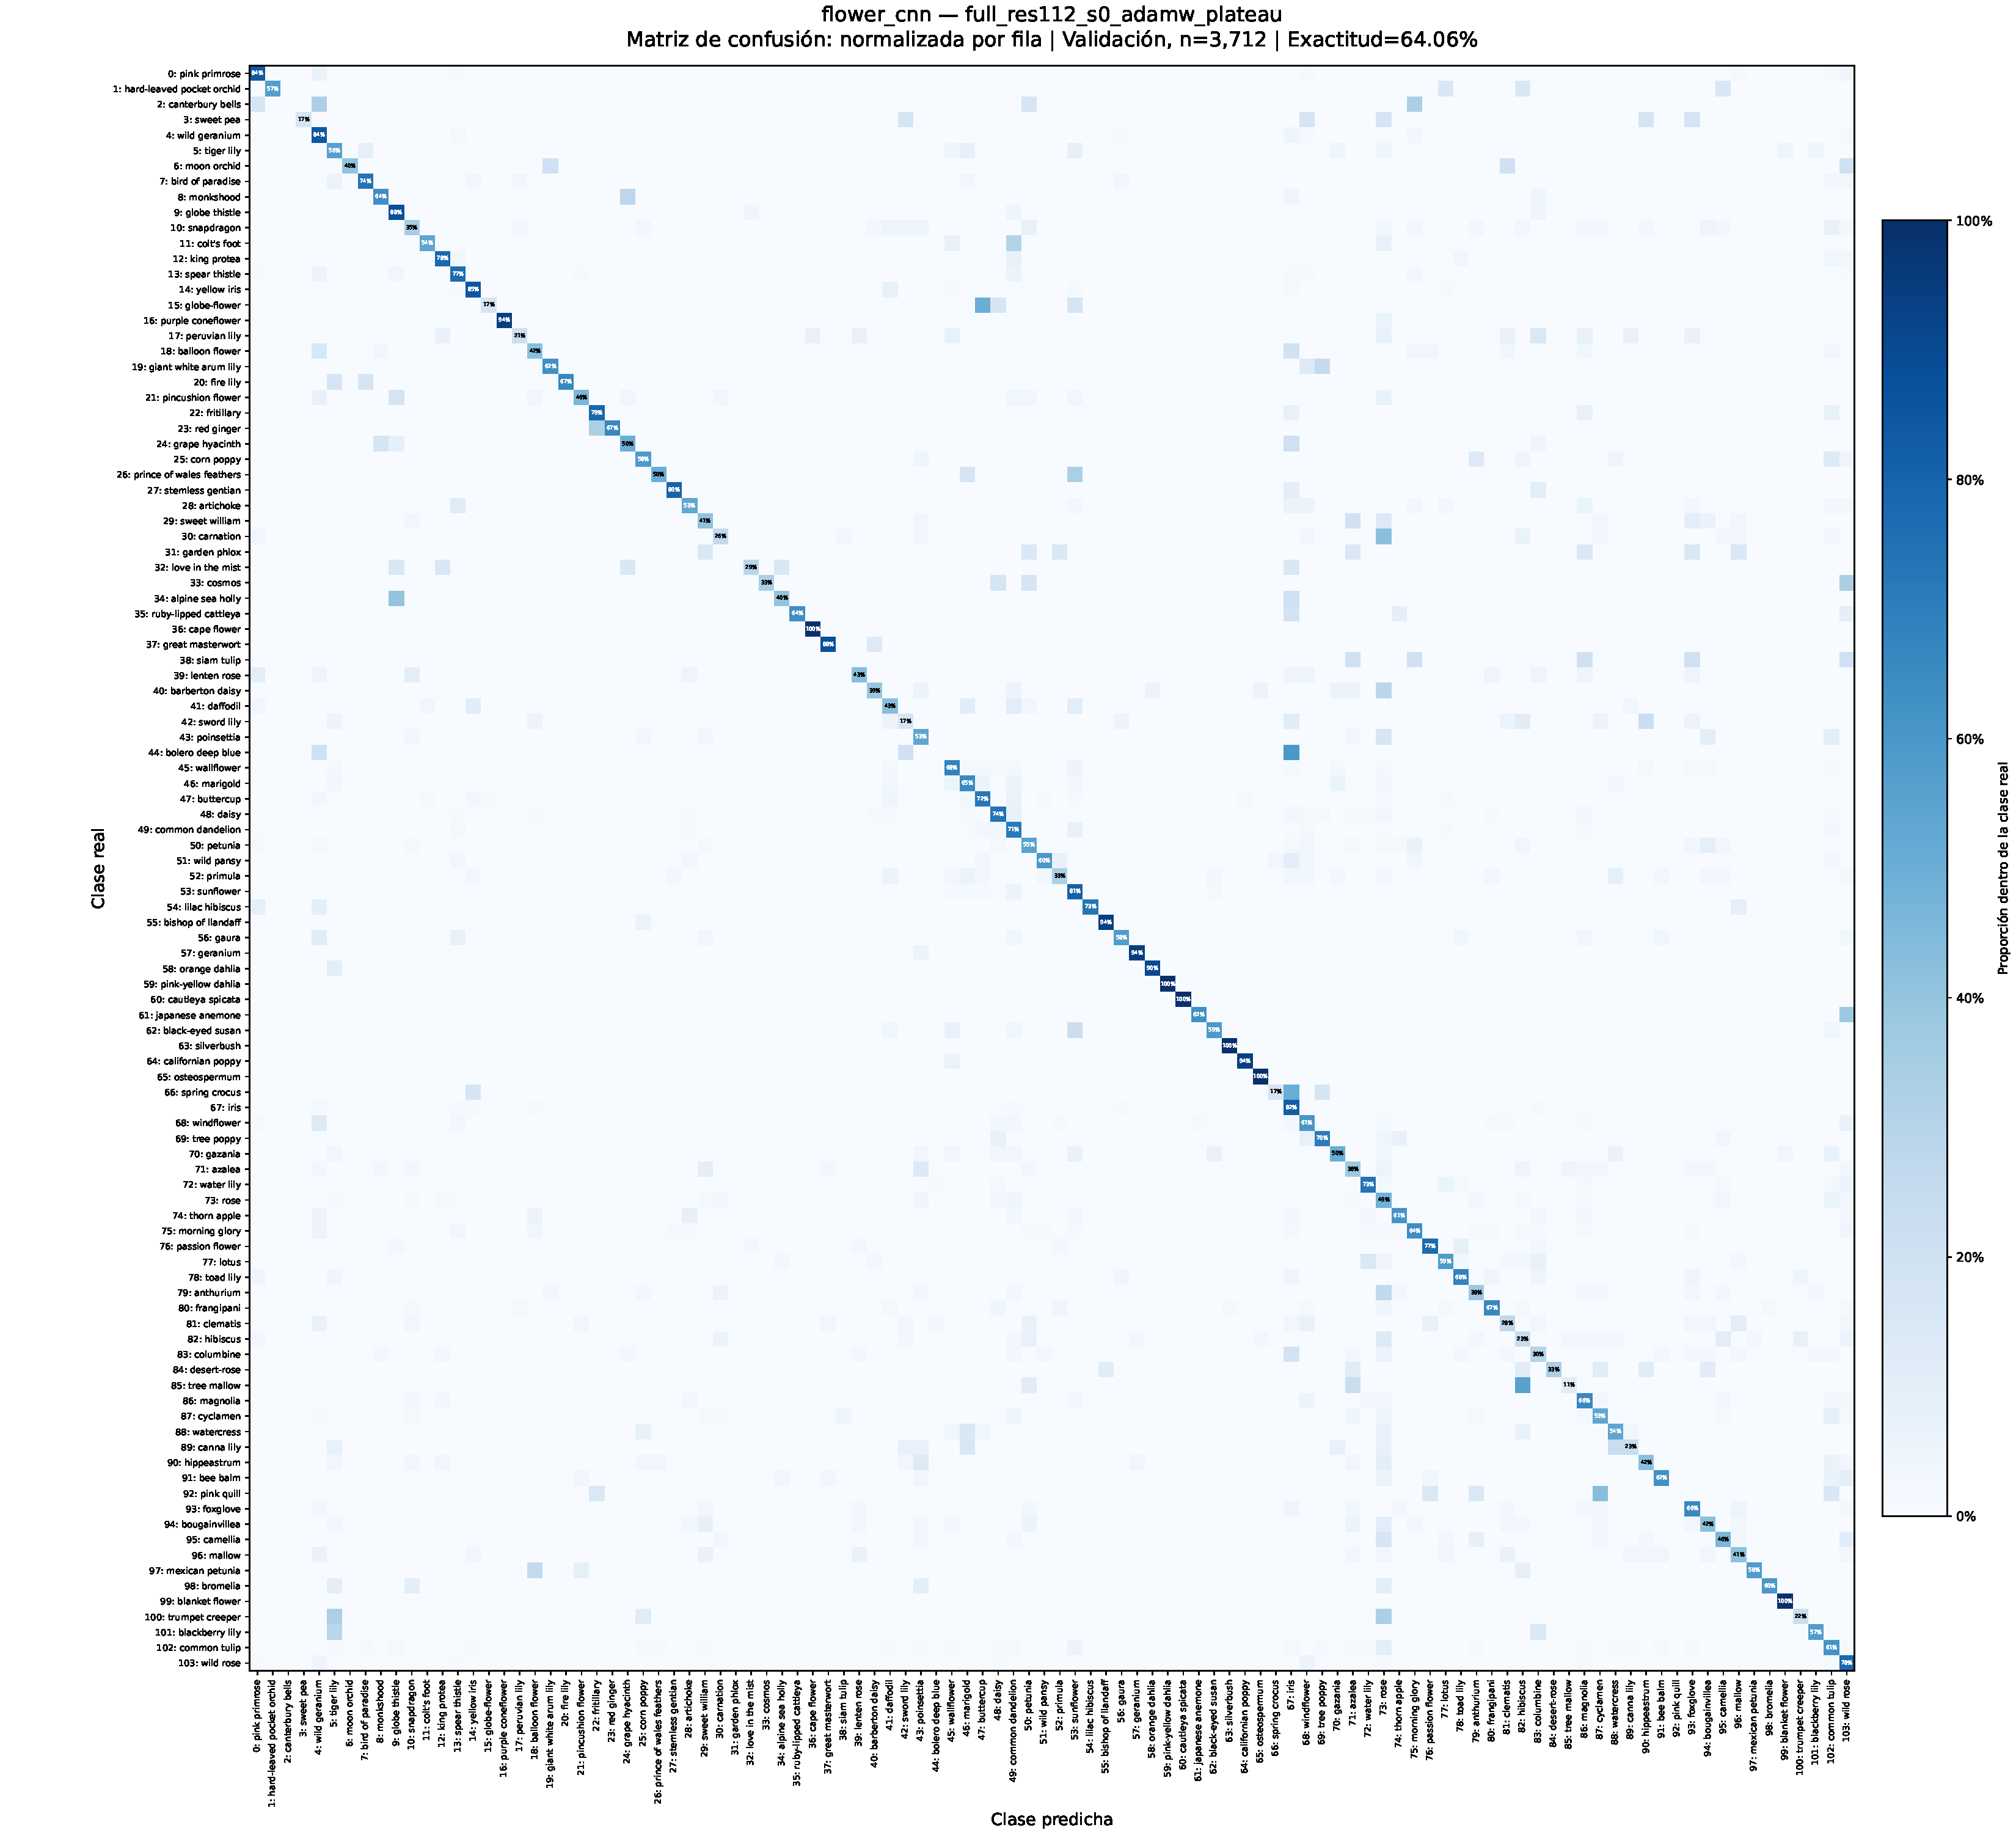
\includegraphics[width=\textwidth,height=0.85\textheight,keepaspectratio]{confusion_referencia.pdf}
\caption{Matriz de confusión normalizada por fila de la CNN de referencia en
validación (104 clases).}
\label{fig:confusion}
\end{figure*}

\subsection{Pesos por clase}
\label{sec:res-class-weight}

La variante con pesos por clase cambia solo la pérdida (Sección~\ref{sec:pesos}): misma
arquitectura, semilla, aumento, dropout y calendario de la tasa. No mejora a la
referencia (Tabla~\ref{tab:desbalance}). Su F1 macro baja de 0.5784 a 0.4881 y
su exactitud de 64.06\% a 48.87\%; 83 de las 104 clases empeoran y solo 17
mejoran.

Los pesos sí hacen lo que se espera de ellos, pero el resultado neto es
negativo. La sensibilidad (\emph{recall}) macro queda igual, 0.56 en ambas
redes, mientras que la precisión macro cae de 0.63 a 0.46: la red no reconoce
mejor las flores, solo reparte sus predicciones de otra manera. Por grupos de
tamaño se ve el intercambio:

\begin{itemize}
\item \textbf{Clases con menos de 30 imágenes (24 clases).} Su sensibilidad
sube de 0.42 a 0.61 y su F1 medio de 0.461 a 0.487. Las clases con F1 = 0
bajan de cinco a dos (\emph{bolero deep blue} y \emph{sweet pea}), y la red
llega a predecir las 104 clases (la referencia nunca predice tres). Pero las
predice de más: a las 10 clases más pequeñas les asigna 112 imágenes de
validación, cuando solo tienen 56 (la referencia les asignaba 25). Su precisión
baja de 0.58 a 0.42, y en esas 10 clases el F1 medio incluso baja un poco (de
0.361 a 0.328), aunque con 5 imágenes de validación por clase esa diferencia
está dentro del ruido.
\item \textbf{Clases con 60 o más imágenes (62 clases).} Pagan el costo. En las
nueve clases de 300 imágenes o más, la sensibilidad cae de 0.72 a 0.40 y el F1
de 0.690 a 0.481; \emph{iris}, por ejemplo, pasa de reconocer 82\% de sus
imágenes a 47\%. Las 44 clases de 60 a 149 imágenes, el grupo más grande, bajan
de 0.530 a 0.405. Como estas clases son mayoría, dominan el promedio macro.
\end{itemize}

Las confusiones cambian de dirección. En la referencia, la flor rara se
confundía con la frecuente (\emph{carnation} $\to$ \emph{rose}, 13 imágenes);
con pesos, ocurre al revés (\emph{rose} $\to$ \emph{carnation}, 15). Los pares
más confundidos son ahora \emph{wild rose} $\to$ \emph{windflower} (28),
\emph{wild geranium} $\to$ \emph{iris} (21) e \emph{iris} $\to$
\emph{wild geranium} (17). La correlación entre tamaño de clase y F1 pasa de
0.12 a $-0.06$ (Figura~\ref{fig:f1-tamano}): la dependencia del tamaño
desaparece, pero porque las clases grandes bajaron, no porque las pequeñas
subieran.

La red con pesos también aprende más despacio. En la época 40, su F1 de
validación es 0.434, contra 0.514 de la referencia, y en el checkpoint (época
70 de 82) su F1 de entrenamiento es 0.638, contra 0.814. Por eso su brecha es
menor (0.150 contra 0.235): no generaliza mejor, ajusta peor el entrenamiento.

Esta configuración se lanzó tres veces; las dos primeras corridas se
interrumpieron por bloqueos de la GPU en las épocas 64 y 68, con un mejor F1 de
0.528 y 0.531. Las tres curvas coinciden hasta la época 40 (F1 de 0.436, 0.429 y
0.434). La corrida completa, que es la que se reporta, recibió su primera
reducción de la tasa en la época 34, contra la 41--42 de las otras dos, y con
ello quedó por debajo. La GPU no es determinista aun con semilla fija, así que
una diferencia de unas 0.04 entre corridas idénticas da una idea del ruido de
una sola semilla. Con cualquiera de las tres, la conclusión es la misma: los
pesos por clase quedan entre 0.05 y 0.09 puntos de F1 por debajo de la
referencia.

\begin{table*}[htbp]
\centering
\caption{Pérdida ponderada por clase frente a la pérdida sin ponderar.}
\label{tab:desbalance}
\small
\begin{tabular}{lrrrrr}
\toprule
Entrenamiento & Exact. (\%) & F1 10 menores & F1 10 mayores & Clases F1 = 0 & F1 macro \\
\midrule
CNN de referencia & 64.06 & 0.3607 & 0.7034 & 5 & \textbf{0.5784} \\
Pesos por clase & 48.87 & 0.3281 & 0.5050 & 2 & 0.4881 \\
\bottomrule
\end{tabular}
\par\smallskip
\parbox{0.95\textwidth}{\footnotesize F1 10 menores/mayores: F1 promedio de las 10 clases con menos (18--19) y más (460--782) imágenes de entrenamiento. Pesos $w_c = N/(K\,n_c)$: van de 0.16 (iris) a 6.81 (las clases de 18 imágenes).}
\end{table*}


\subsection{Efecto de la regularización}
\label{sec:res-regularizacion}

Para medir qué aportan las técnicas de regularización, se entrenó la misma CNN,
con la misma semilla y el mismo tope de épocas, sin dropout, sin aumento de
datos y con Adam en lugar de AdamW (Tabla~\ref{tab:regularizacion} y
Figura~\ref{fig:curvas-regularizacion}). Sin regularización, la red aprende más
rápido al principio: llega a un F1 de validación de 0.5 en la época 25, frente a
la 38 de la referencia. Pero ahí se estanca. Su mejor F1 es 0.5332, 0.045 por
debajo de la referencia (0.5784), y su exactitud baja de 64.06\% a 59.64\%.

La causa es el sobreajuste. Sin regularización, el F1 de entrenamiento sube a
0.877 (0.814 con regularización) y la brecha de F1 pasa de 0.235 a 0.344. La
pérdida de validación toca su mínimo en la época 25 (1.825) y después sube hasta
2.122, mientras que con regularización su mínimo es 1.464 y prácticamente no
sube. El daño se concentra en las clases pequeñas: el F1 promedio de las 10
clases más pequeñas baja de 0.361 a 0.257, mientras que el de las 10 más grandes
solo baja de 0.703 a 0.669. Las clases con 18--30 imágenes son las más fáciles
de memorizar y, sin aumento, la red ve siempre las mismas pocas fotos.

\begin{table*}[htbp]
\centering
\caption{La misma CNN con y sin regularización (semilla 0, mismas épocas máximas).}
\label{tab:regularizacion}
\small
\begin{tabular}{lcccrrrrr}
\toprule
Variante & Dropout & Aumento & Pesos & Época & Exact. (\%) & F1 entr. & Brecha F1 & F1 macro \\
\midrule
CNN de referencia & 0.5 & sí & WD 0.01 & 91/103 & 64.06 & 0.8138 & +0.2354 & \textbf{0.5784} \\
Sin regularización & 0 & no & -- & 34/46 & 59.64 & 0.8767 & +0.3435 & 0.5332 \\
\bottomrule
\end{tabular}
\par\smallskip
\parbox{0.95\textwidth}{\footnotesize Pesos: WD = weight decay desacoplado de AdamW; -- = Adam sin decaimiento. Ambas comparten arquitectura, tasa de aprendizaje inicial, reducción de LR en meseta, paciencia de 12 evaluaciones y tope de 150 épocas.}
\end{table*}


\begin{figure*}[htbp]
\centering
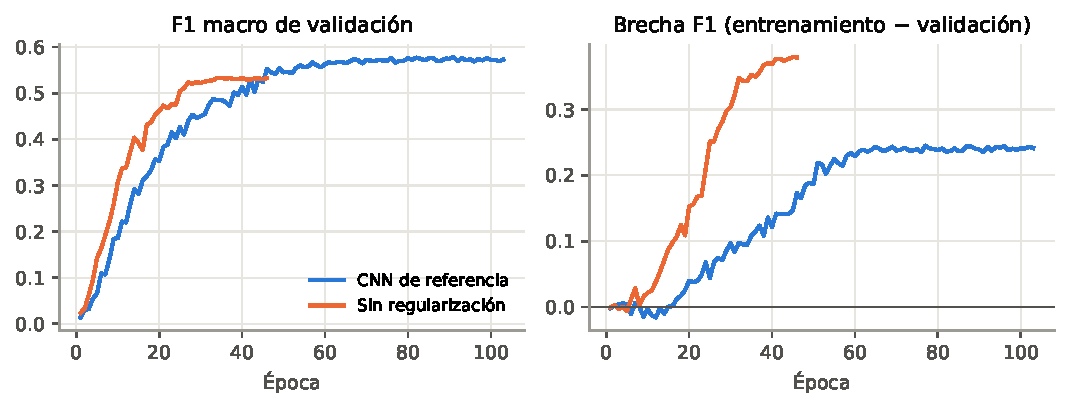
\includegraphics[width=0.85\textwidth]{curvas_regularizacion.pdf}
\caption{F1 macro de validación y brecha de F1 por época, con y sin
regularización (misma semilla, arquitectura y tope de épocas).}
\label{fig:curvas-regularizacion}
\end{figure*}

\subsection{Hiperparámetros}
\label{sec:res-hiperparametros}

La Tabla~\ref{tab:hiperparametros} cambia un hiperparámetro a la vez respecto
a la referencia, con el conjunto completo de entrenamiento. Ninguna de las dos
variantes la mejora:

\begin{itemize}
\item \textbf{Tasa de aprendizaje de $3\times10^{-4}$ (en vez de
$10^{-3}$): F1 0.4605.} Es la peor de las CNN, pero no por sobreajuste: su brecha
de F1 es solo 0.094 porque la red tampoco aprende bien el entrenamiento (F1 de
entrenamiento 0.554, contra 0.814 de la referencia). La reducción automática de
la tasa ocurre cuando la pérdida de validación deja de mejorar dos épocas; al
partir de una tasa ya baja, en pocas reducciones llega al mínimo de $10^{-5}$ y
el aprendizaje prácticamente se detiene. En la época del checkpoint (98) la tasa
ya estaba en ese mínimo. Es infraajuste causado por el calendario de la tasa, no
por la capacidad de la red.
\item \textbf{Dropout de 0.3 (en vez de 0.5): F1 0.5596.} Con menos dropout,
el F1 de entrenamiento es prácticamente igual (0.816 contra 0.814), pero el de
validación baja 0.019 y la brecha sube de 0.235 a 0.256. Es el mismo patrón que
sin regularización, en menor grado: menos regularización, más memorización. De
nuevo, las clases pequeñas son las que más pierden (0.286 contra 0.361).
\end{itemize}

Con una sola semilla, la diferencia de 0.019 del dropout es moderada; la de la
tasa de aprendizaje (0.118) es clara.

\begin{table*}[htbp]
\centering
\caption{Efecto de un hiperparámetro a la vez, con el conjunto completo.}
\label{tab:hiperparametros}
\small
\begin{tabular}{lcccrrrrr}
\toprule
Configuración & LR & Dropout & Resolución & Época & Exact. (\%) & Brecha F1 & Tiempo (min) & F1 macro \\
\midrule
CNN de referencia & 0.001 & 0.5 & 112 & 91/103 & 64.06 & +0.2354 & 19.7 & \textbf{0.5784} \\
LR $3\times10^{-4}$ & 0.0003 & 0.5 & 112 & 98/110 & 54.18 & +0.0936 & 22.5 & 0.4605 \\
Dropout 0.3 & 0.001 & 0.3 & 112 & 61/73 & 61.96 & +0.2561 & 15.0 & 0.5596 \\
\bottomrule
\end{tabular}
\par\smallskip
\parbox{0.95\textwidth}{\footnotesize Cada fila cambia un solo valor respecto a la referencia (LR $10^{-3}$, dropout 0.5, 112$\times$112).}
\end{table*}


\subsection{Reducción de datos con Distribution Matching}
\label{sec:res-dm}

Como experimento independiente de los anteriores, se evaluó si un conjunto
pequeño de imágenes sintéticas generado con Distribution Matching (DM)
\autocite{zhao2023dm} conserva
más información que el mismo número de imágenes reales elegidas al azar
(Tabla~\ref{tab:dm}). Con una imagen por clase (IPC 1, 104 imágenes), DM supera
a la selección aleatoria (F1 0.067 frente a 0.051). Con diez por clase
(IPC 10, 1,040 imágenes) ocurre lo contrario: las imágenes reales dan 0.258 y
las sintéticas 0.204, con más variación entre semillas. La destilación ayuda
solo cuando hay muy pocas imágenes, y su costo (16 y 25 minutos de generación)
se suma al del entrenamiento. Ninguna de estas imágenes se usó en los demás
experimentos; todos entrenan con las 12,753 imágenes reales.

\begin{table}[htbp]
\centering
\caption{Selección aleatoria frente a destilación con Distribution Matching (DM).}
\label{tab:dm}
\small
\begin{tabular}{rrlrrr}
\toprule
IPC & Imágenes & Conjunto & Exact. (\%) & F1 macro & Destilación (min) \\
\midrule
1 & 104 & Sintéticas (DM) & 9.85 & 0.0672 $\pm$ 0.0052 & 16 \\
1 & 104 & Reales aleatorias & 5.75 & 0.0514 $\pm$ 0.0029 & -- \\
10 & 1,040 & Sintéticas (DM) & 20.55 & 0.2044 $\pm$ 0.0235 & 25 \\
10 & 1,040 & Reales aleatorias & 25.86 & 0.2575 $\pm$ 0.0082 & -- \\
\bottomrule
\end{tabular}
\par\smallskip
\parbox{0.95\textwidth}{\footnotesize Promedio $\pm$ desviación estándar de tres semillas de entrenamiento por condición. Misma CNN, Adam $10^{-3}$, $112\times112$. Datos: \path{reports/resultados.csv}.}
\end{table}



\section{Análisis}
\label{sec:analisis}

\subsection{Por qué la CNN supera a la MLP}

La diferencia entre la MLP (F1 0.018) y la CNN de referencia (F1 0.578) no es de
grado sino de tipo: la MLP no logra ajustar ni siquiera el entrenamiento
(F1 de entrenamiento 0.019), mientras que la CNN sí lo ajusta y luego
generaliza parcialmente. La causa está en cómo cada red trata la imagen.

\begin{itemize}
\item \textbf{La MLP no comparte pesos.} Aplana la imagen en 37,632 valores y
conecta cada uno con cada neurona oculta: el 99.7\% de sus 9.66 millones de
parámetros está en esa primera capa. Un pétalo en la esquina superior y el mismo
pétalo en el centro activan pesos distintos, así que la red tendría que aprender
cada patrón por separado en cada posición. Con 122 imágenes por clase en
promedio, no hay datos suficientes para eso.
\item \textbf{La CNN codifica supuestos correctos sobre imágenes.} Sus filtros
de $3\times3$ miran vecindarios locales y se aplican en toda la imagen (pesos
compartidos), las capas sucesivas combinan bordes en texturas y texturas en
partes, y el \emph{pooling} global hace que la predicción dependa de qué hay en
la imagen y no de dónde está. Con 20 veces menos parámetros (480,936) aprovecha
mucho mejor los mismos datos.
\item \textbf{La MLP se refugia en las clases grandes.} Solo predice 11 clases y
su F1 por clase sí depende fuertemente del tamaño de la clase (Spearman 0.51,
frente a 0.12 en la CNN): sin poder distinguir flores, lo mejor que encuentra es
favorecer las clases más frecuentes. Además es inestable: con la tasa de
$10^{-3}$ de la CNN colapsa a una sola clase, por lo que necesitó $10^{-4}$.
\end{itemize}

La comparación no aísla por completo el efecto de las convoluciones: las dos redes
difieren también en número de parámetros y la MLP usa una tasa de aprendizaje
diez veces menor. Aun así, una diferencia de 0.56 puntos de F1 macro con la
misma política de entrenamiento, los mismos datos y el mismo aumento no se
explica por la tasa: con la tasa de la CNN, la MLP es todavía peor.

Los regularizadores no son el problema de la MLP: su curva con aumento y dropout
(gris en la Figura~\ref{fig:curvas-modelos}) es todavía peor que la limpia, y su
brecha es nula. Regularizar más una red que infraajusta no la ayudaría.

\subsection{Por qué la CNN más profunda empeoró}

Agregar dos convoluciones (de 480,936 a 1,218,600 parámetros) bajó el F1 de
0.578 a 0.566. Con una sola semilla, una diferencia de 0.012 es pequeña, pero
coincide con el Avance~4 (0.574 contra 0.550) y las curvas explican por qué la
red más grande no mejora:

\begin{itemize}
\item \textbf{Más capacidad sin más datos.} La red ampliada ajusta el
entrenamiento mucho más rápido: en la época 41 su F1 de entrenamiento es 0.794,
contra 0.638 de la referencia, pero su F1 de validación se estanca en 0.564. La
capacidad extra se usa para memorizar detalles del entrenamiento, sobre todo en
las clases con 18--30 imágenes, no para aprender rasgos que generalicen.
\item \textbf{El sobreajuste aparece antes.} Su pérdida de validación toca su
mínimo en la época 34 (frente a la 54 de la referencia) y después sube, y tiene
seis clases con F1 = 0 en vez de cinco.
\item \textbf{La regularización estaba calibrada para la red pequeña.} Ambas
usan dropout 0.5 y decaimiento de pesos de 0.01. Para una red con 2.5 veces más
parámetros, esa misma regularización es relativamente más débil.
\item \textbf{Más profundidad no agrega información a $112\times112$.} Las dos
capas nuevas operan sobre mapas ya reducidos; a esa resolución, los detalles
finos que distinguen flores parecidas (\emph{carnation} contra \emph{rose}) ya se
perdieron en la entrada, y ninguna capa extra los recupera.
\end{itemize}

En resumen, el cuello de botella de este problema no es la capacidad del modelo
sino la cantidad de datos por clase. Por eso los cambios que atacan la falta de
datos, como el aumento, tienen más efecto que hacer la red más grande.

\subsection{Qué aporta la regularización}

Los tres experimentos de regularización apuntan en la misma dirección: quitar
regularización (Sección~\ref{sec:res-regularizacion}) o reducirla (dropout 0.3)
sube el F1 de entrenamiento o lo deja igual, pero baja el de validación y abre
la brecha. Con 12,753 imágenes y 480,936 parámetros, la CNN tiene capacidad de
sobra para memorizar el entrenamiento; la regularización es la que le permite
generalizar. Su efecto conjunto vale 0.045 puntos de F1 macro.

La regularización no elimina el sobreajuste: la referencia conserva una brecha
de 0.235. Las curvas muestran que la brecha se estabiliza alrededor de la época
60, justo cuando la reducción automática de la tasa lleva el aprendizaje casi a
cero. A partir de ahí la red deja de cambiar, en vez de seguir memorizando. Esto
también explica por qué la referencia toma su mejor checkpoint tan tarde (época
91): son ajustes finos con una tasa de $10^{-5}$.

\subsection{Sensibilidad a los hiperparámetros}

La tasa de aprendizaje es, de lejos, el hiperparámetro más sensible: bajarla a
$3\times10^{-4}$ cuesta 0.118 de F1, más que quitar toda la regularización. La
causa es la interacción con la reducción en meseta: una tasa inicial baja hace
que el calendario la lleve al mínimo antes de que la red aprenda lo suficiente.
Con este calendario, $10^{-3}$ es la elección correcta. El dropout es menos
sensible: entre 0.3 y 0.5 la diferencia es de 0.019, a favor de 0.5.

% PENDIENTE: desbalance (class_weight)

\subsection{Limitaciones}

Cada configuración se entrenó con una sola semilla, por lo que diferencias de
menos de unas centésimas de F1 no deben tomarse como concluyentes. La
validación se usó para elegir el checkpoint de cada corrida, lo que sesga sus
métricas ligeramente hacia arriba; los puntajes de Kaggle
(Sección~\ref{sec:kaggle}) son la única medida sobre datos nunca vistos. La
corrida de la CNN ampliada se interrumpió en la época 50. Todas las redes se
entrenaron desde cero a $112\times112$; no se evaluó transferencia de
aprendizaje desde modelos preentrenados.

\section{Conclusiones}
\label{sec:conclusiones}

El mejor modelo de este trabajo es la CNN de referencia: cuatro convoluciones,
480,936 parámetros, dropout de 0.5, aumento de datos, AdamW y reducción de la
tasa en meseta. En validación alcanza un F1 macro de 0.5784 y una exactitud de
64.06\%. Ninguno de los seis cambios evaluados, cada uno aislado respecto a ella,
la superó.

Las preguntas que planteaba el trabajo tienen respuestas claras:

\begin{itemize}
	\item \textbf{¿Ayuda extraer patrones espaciales?} Sí, y de forma decisiva. La
	      MLP, con 20 veces más parámetros, no logra ajustar ni el entrenamiento (F1 de
	      0.018). Compartir filtros locales en toda la imagen es lo que hace aprendible el
	      problema con unas cien imágenes por clase.
	\item \textbf{¿Ayuda una red más profunda?} No. La CNN ampliada memoriza el
	      entrenamiento más rápido, pero su validación se estanca en el mismo nivel (F1
	      de 0.566). Con una sola semilla, su diferencia con la referencia está dentro del
	      ruido; lo que sí muestra es que, con estos datos, agregar capas no basta para subir
	      el techo.
	\item \textbf{¿Ayuda la regularización?} Sí. Sin dropout, aumento ni
	      decaimiento de pesos, la brecha de F1 sube de 0.235 a 0.344 y el F1 de
	      validación baja 0.045, con la mayor pérdida en las clases pequeñas. Reducir el
	      dropout a 0.3 va en la misma dirección.
	\item \textbf{¿Ayuda compensar el desbalance con pesos por clase?} No. Sube la
	      sensibilidad de las clases raras, pero a costa de predecirlas de más y de
	      perder las clases medianas y grandes, que son mayoría; el F1 macro baja a
	      0.488.
	\item \textbf{¿Qué tan sensibles son los hiperparámetros?} La tasa de
	      aprendizaje es el más sensible: con $3\times10^{-4}$, el calendario en meseta la
	      lleva al mínimo antes de que la red aprenda, y el F1 baja a 0.461.
\end{itemize}

En conjunto, los experimentos muestran un techo cercano a 64\% de exactitud con
dos causas que actúan juntas: la capacidad limitada de una CNN pequeña entrenada
desde cero y la falta de datos por clase, que impide que más capas se traduzcan
en rasgos útiles. Lo que ataca la falta de datos, como el aumento, ayuda; lo que
agrega capas sin más datos o solo redistribuye las predicciones, no. El análisis de
errores lo confirma: los fallos se concentran en flores parecidas entre sí
(\emph{carnation} y \emph{rose}, \emph{wild rose} y \emph{windflower}) y en las
24 clases con menos de 30 imágenes, donde a $112\times112$ los detalles que las
distinguen se pierden.

Frente al Avance~4, este reporte corrige la forma de medir el sobreajuste. Al
evaluar el entrenamiento sin aumento ni dropout, la brecha real de la referencia
resulta casi el doble de la reportada antes. Además, todo el proceso es
reproducible: el notebook reconstruye la tabla de resultados, las tablas y las
figuras a partir de los historiales versionados de cada corrida.

\subsection{Trabajo futuro}

El paso con más potencial es la transferencia de aprendizaje: una red
preentrenada en ImageNet (por ejemplo, EfficientNetB0 o ResNet50) a
$224\times224$ aporta rasgos aprendidos de millones de imágenes, que es justo lo
que falta aquí, y la resolución mayor conserva los detalles que separan flores
parecidas. Para el desbalance, conviene probar pesos más suaves o corregir los
umbrales de decisión después de entrenar, en lugar de pesos inversamente
proporcionales al tamaño. Por último, repetir cada configuración con varias
semillas permitiría decidir las diferencias pequeñas que hoy quedan dentro del
ruido, como las de la CNN ampliada y el dropout.

\section{Conclusión individual (Angel Luna)}

Este proyecto me permitió comprobar, con evidencia experimental y no solo con intuición teórica, qué factores determinan realmente el desempeño de una red neuronal en un problema de clasificación de imágenes con pocos datos por clase. Con una CNN de referencia de cuatro convoluciones y 480,936 parámetros se obtuvo un F1 macro de 0.5784 y una exactitud de 64.06,\% en validación. Ninguno de los seis cambios evaluados, cada uno aislado respecto a ella, logró superarla.

El resultado que considero más instructivo es la comparación entre la MLP y la CNN. Con veinte veces más parámetros, la MLP alcanzó un F1 de apenas 0.018 y no pudo ajustar ni el entrenamiento. Se sigue que lo decisivo no es el número de parámetros, sino que la arquitectura incorpore el supuesto correcto sobre los datos: los filtros locales con pesos compartidos hacen aprendible el problema con alrededor de cien imágenes por clase. Esto me dejó claro que la capacidad de un modelo debe entenderse junto con su sesgo inductivo y no de forma aislada.

También aprendí que más capacidad no implica mejor generalización. La CNN ampliada memorizó el entrenamiento más rápido, pero su validación se estancó en el mismo nivel (F1 de 0.566). Del mismo modo, los pesos por clase, que en principio parecen una solución natural al desbalance, redujeron el F1 macro a 0.488: la sensibilidad macro no cambió y la precisión cayó, es decir, la red solo redistribuyó sus predicciones en lugar de distinguir mejor las flores. En cambio, la regularización sí aportó (el F1 de validación bajó 0.045 al retirarla y la brecha de F1 subió de 0.235 a 0.344), y la tasa de aprendizaje resultó ser el hiperparámetro más sensible por su interacción con la reducción en meseta.

Un aprendizaje metodológico importante fue corregir la forma de medir el sobreajuste. Al evaluar el entrenamiento sin aumento de datos y sin dropout, la brecha real resultó casi el doble de la reportada en el avance anterior. Aprendí que una métrica solo es comparable cuando se mide bajo las mismas condiciones, y que una conclusión puede cambiar por completo según cómo se calcule.

Reconozco también las limitaciones del trabajo. Cada configuración se entrenó con una sola semilla y las corridas repetidas de los pesos por clase mostraron una variación de aproximadamente 0.04 en F1, por lo que diferencias pequeñas, como la de la CNN ampliada o la del dropout, no son concluyentes. Además, la validación se usó para elegir el checkpoint y no se evaluó sobre datos nunca vistos. Con estas salvedades, las diferencias grandes (MLP, tasa de aprendizaje y pesos por clase) sí son sólidas.

Finalmente, los resultados señalan un techo cercano a 64,\% de exactitud con dos causas que actúan juntas: la capacidad limitada de una CNN pequeña entrenada desde cero a $112 \times 112$ y la escasez de datos por clase. Por ello, el siguiente paso natural es la transferencia de aprendizaje desde un modelo preentrenado en ImageNet, junto con repetir los experimentos con varias semillas. Más allá de la cifra final, el proyecto me deja una forma de trabajo que considero valiosa: cambiar un solo factor a la vez, medir con cuidado y no atribuir a una mejora lo que podría ser ruido.


\clearpage
\printbibliography[title={Referencias}]
\end{document}
